\documentclass[master]{thesis-uestc}
\usepackage{tikz} % 必须的基础绘图包

% 此处-----------|---的模板类型设置请参照README
\title{大功率宽频带脊波导微波窗研究}{English Title} % 论文题目
\author{方源}{English Name} % 作者姓名
\setdate[submit]{ } % 论文提交日期,可留空
\setdate[oral]{ }  % 答辩日期,可留空
\setdate[confer]{ } % 学位授予日期,可留空
\advisor{\qquad 王建勋\qquad\qquad 教\chinesespace 授}{English name English title}
% \coAdvisor{合作导师姓名\chinesespace 导师职称}{Co advisor English name English title} % 仅专业硕士/博士使用,在扉页/英文首页添加合作导师,不使用请注释
\school{电子科学与工程学院}{School of Electronic Science and Engineering} % 学院信息
\major{电子科学与技术}{Electronic Science and Technology} % 专业信息
\studentnumber{202221020122} % 学号
\ProfessionalDegreeArea{随便学学} % 专业硕士专用:专业学位领域
\ClassificationNumber{TP309.2} % 分类号
\ClassifiedClass{公开} % 密级
\UDCNumber{004.78} % UDC号
\Chairman{xxxxx} % 答辩委员会主席

% 取消注释以下内容,用于禁止文中换行处的英语单词自动截断换行。
% \tolerance=1
% \emergencystretch=\maxdimen
% \hyphenpenalty=10000
% \hbadness=10000

\makeglossaries % 产生缩略词表/符号表专用,不使用时请注释。 注意,之后的acronym,glossaryentry以及相关的引用也请注释。
\newacronym[description=逻辑卷管理器]{lvm}{LVM}{Logical Volume Manager} % 定义缩略词:以本项为例,逻辑卷管理器为中文名称;lvm用于文内引用;LVM为显示的应为缩略语或符号;Logical Volume Manager为显示的英文全称/描述。
\newglossaryentry{tree}{name={tree}, description={trees are the better humans}}  % 定义符号:以本项为例,name={tree}为符号名称;tree用于文内引用; description={trees are the better humans}为显示的描述。页码自动添加。

\begin{document}

\makecover % 封面+中英文扉页
\originalitydeclaration % 原创新声明
% \signatureofdeclaration{signature.pdf} % 用于添加扫描版签字后的原创新声明(使用时取消注释本行,并注释掉上一行)
% 中文摘要
\begin{chineseabstract}

    \chinesekeyword{xxx,xxx,xxx} % 中文关键词
\end{chineseabstract}
% 英文摘要
\begin{englishabstract}

    \englishkeyword{xxx, xxx, xxx} % 英文关键词
\end{englishabstract}

\thesistableofcontents % 目录
\thesisfigurelist % 图目录,仅在需要时添加,一般情况下请注释
\thesistablelist % 表目录,仅在需要时添加,一般情况下请注释
% \glsaddall % 默认仅显示被正文引用的项,取消注释以显示所有已定义的缩略词/符号
\thesisglossarylist % 缩略词表,仅在需要时添加,一般情况下请注释
\thesissymbollist % 符号表,仅在需要时添加,一般情况下请注释

% 正文内容


\chapter{绪\hspace{6pt}论}
\section{生活中的微波真空管器件}
\section{真空管的微波窗}
\section{真空管中的宽带宽需求}
\section{国内外研究现状}

\section{论文结构与安排}
\chapter{微波窗的理论研究}


\section{微波等效电路分析}
为了寻求复杂的微波系统的传输特性,可以将其划分为均匀导波系统和非均匀微波元器件构成的复杂边界系统。通过使用传输线方程和结合实际的端接条件等数学手法,传输特定模式的电磁场的均匀导播系统可以被转化为传输线这一电路模型。由于相比于直接使用电磁场进行分析,电路相关的分析理论较为成熟,这一转化思想为分析复杂微波传输系统提供了良好的基础。
\subsection{常见微波传输线的特性阻抗}
在进行等效电路分析的时候,无论是进行阻抗匹配或者阻抗变换的设计还是进行特定的滤波器等无源器件的设计,,传输线的特性阻抗\(Z_C\)是一个非常重要的参数。现在先对常见的微波传输线的特性阻抗进行相应的分析。

同轴线是一种非常常见的传输线,其主要传输的模式是\(TEM\)模式,这种模式能够传输直流相关的信号,故其截止频率为0Hz。并且由于同轴线的次高模式的截止频率较高,此时同轴线的带宽也较宽。通过对同轴线上面的传输的基本模式\(TEM\)模式的电场与磁场进行相应的积分,可以求出其相应的特性阻抗\(Z_C\),其表达式为\ref{eq:同轴线的特性阻抗}。
\begin{equation}\label{eq:同轴线的特性阻抗}
    Z_C = \frac{60}{\sqrt{\epsilon_r}} \ln \left( \frac{b}{a} \right)
\end{equation}
式子中,\(b, a\)分别为同轴线的外径和内径,\(\epsilon_r\)为同轴线填充均匀材料时的相对介电常数。但是在实际的应用过程中,为了兼顾同轴线系统的损耗与功率容量等因素的考虑,通常会将同轴线的特性阻抗\(Z_C\)取为\(50 \Omega\),这也是很多标准同轴线的特性阻抗。

矩形波导也是一种常见的微波传输线,但是由于矩形波导的基本模式\(TE_{10}\)模式为\(TE\)模式,为了计算特性阻抗,对其传输模式的电场与磁场进行积分时候无法像\(TEM\)模式一样进行出现单值积分。故矩形波导以及后续传输非\(TEM\)模式的波导的特性阻抗结果都不唯一。具体的定义方法可以被分为电压-电流定义、功率-电压定义以及功率-电流定义。由于后续应用主要使用的是功率-电压定义,故本文如果不进行特别说明的话特性阻抗主要使用的便是功率-电压定义的特性阻抗\(Z_{P, U}\),此时根据文献\cite{heihil_characteristic_2006}中的定义,矩形波导的特性阻抗可以被表示为
\subsection{脊波导的工作特性与工作参数}\label{subsec:DoubleRidgeTheory}
脊波导作为一种常见的宽带传输线,针对其主要的理论分析方法是横向谐振法(Transverse Resonance Method, TRM)。根据参考文献\citing{helszajn_double_ridge_2000, pingwang_double_ridge_2004,pingyingjiang_double_ridge_2007,hopefer_design_ridge_1955}使用横向谐振法可以分析出脊波导的截止频率、主模带宽以及其特性阻抗。需要注意的是,本文主要涉及以及本小节主要分析的脊波导为脊位于矩形波导长边或者短边正中间的对称情况,如果有不对称脊波导的需求的话,可以参考文献\cite{ramesh_asymmetri_2001}中的求解方法进行分析。

脊波导传输的基本模式是主模类$TE_{10}$模式,其次高模式为类$TE_{20}$模式,为了分析这两个模式的截止频率,有必要画出脊波导在横向上的等效电路。其中,脊两边的空隙可以分别被等效为两端传输线,脊凸起的平台也可以被等效为一段传输线,凸起的脊的两侧所引入的不连续性由于会与对侧的脊或者底边产生电势差,故可以分别被等效为两端电容。当模式截止时,根据横向谐振法,相当于横向的等效电路陷入谐振情况。此时以脊的左侧为参考平面,假设向左看得到的等效导纳为$Y_{1}$,向右看得到的等效导纳为$Y_{2}$,如果产生了横向谐振那么可以得到横向谐振方程\ref{eq:Y1Y2}:
\begin{equation}\label{eq:Y1Y2}
    Y_{1}=-Y_{2}
\end{equation}

以此为基础,我们可以得到分析脊波导的截止频率的横向谐振方程\ref{eq:TRM_DW}:
\begin{equation}\label{eq:TRM_DW}
    -\cot \theta_1 + \left( \frac{Y_{02}}{Y_{01}} \right) \tan \theta_2 + \frac{B}{Y_{01}} = 0 
\end{equation}
其中参数可被表示为等式\ref{eq:TRM_DW_parameters}中的\ref{eq:Y01}到\ref{eq:BY01}:
\begin{subequations}\label{eq:TRM_DW_parameters}
    \begin{align}
    Y_{01} &= \frac{k_c}{\omega \mu_0} \left( \frac{1}{b} \right) \label{eq:Y01} \\
    Y_{02} &= \frac{k_c}{\omega \mu_0} \left( \frac{1}{d} \right) \label{eq:Y02} \\
    \theta_1 &= \frac{\pi (a - s)}{\lambda_c} = \pi \left( 1 - \frac{s}{a} \right) \left( \frac{a}{\lambda_c} \right) \label{eq:theta1} \\
    \theta_2 &= \frac{\pi s}{\lambda_c} = \pi \left( \frac{s}{a} \right) \left( \frac{a}{\lambda_c} \right) \label{eq:theta2} \\
    \frac{B}{Y_{01}} & \approx 2 \delta_{r} \left( \frac{b}{a} \right) \left( \frac{a}{\lambda_c} \right) \ln \csc \left( \frac{\pi d}{2b} \right) \label{eq:BY01}
    \end{align}
\end{subequations}
式子\ref{eq:TRM_DW_parameters}中的参数定义如下:$a$为脊波导长边长,$b$为脊波导短边长,$s$为脊的宽度,$d$为脊凸起后留下的空腔缝隙宽度。$\delta_{r}$为与脊波导相关的几何系数:双脊波导时$\delta_{r}=1$,单脊波导时$\delta_{r}=2$。$\omega$为当前角频率;$\mu_0$为真空磁导率。波导截止波数$k_c=2\pi / \lambda_c$,截止波长$\lambda_c$在真空填充脊波导时与截止频率$f_c$满足$\lambda_c=c/f_c$。$Y_{01}$为脊两侧空腔所引入的导纳,$Y_{02}$为脊所引入的导纳,$\frac{B}{Y_{01}}$为脊引入电纳按照$Y_{01}$进行归一化之后的结果。

此时如果式子\ref{eq:BY01}中的对数函数套三角函数造成超越方程以至于难以求解,可以使用近似替代公式\ref{eq:ln_csc}:
\begin{equation}
    \ln \csc \left( \frac{\pi \alpha}{2} \right) \approx \frac{1}{2} \left[ \left( \frac{1 + \alpha^2}{\alpha} \right) \ln \left( \frac{1 + \alpha}{1 - \alpha} \right) - 2 \ln \left( \frac{4 \alpha}{1 - \alpha^2} \right) \right] \label{eq:ln_csc}
\end{equation}
其中,$\alpha=d/b$,为脊的空隙与脊波导短边之比。

关于双脊波导的截止频率有近似的显式解\citing{Hoefer1982AnalyticalEF},如果双脊波导的几何形状满足以下约束关系\ref{eq:DRW_constraints}:
\begin{equation}\label{eq:DRW_constraints}
    \begin{aligned}
    0.01 &\leq \frac{d}{b} \leq 1 \\
    0 &\leq \frac{b}{a} \leq 1 \\
    0 &\leq \frac{s}{a} \leq 0.45
    \end{aligned}
\end{equation}
使用式子\ref{eq:DRW_closed}求解时候的误差小于1\%

\begin{equation}\label{eq:DRW_closed}
    \begin{split}
        \frac{a}{\lambda_c} = \frac{a}{2(a - s)} & \left[ 1 + \frac{4}{\pi} \left( 1 + 0.2 \sqrt{\frac{b}{a - s}} \right) \left( \frac{b}{a - s} \right) \ln \csc \left( \frac{\pi d}{2b} \right) \right. \\
        & \left. + \left( 2.45 + 0.2 \frac{s}{a} \right) \left( \frac{sb}{d(a - s)} \right) \right]^{-\frac{1}{2}}
    \end{split}
\end{equation}

配合MATLAB或者Mathematica等数学软件,可以对以上式子进行数值求解,进而得到给定几何参数下的脊波导的截止频率。这些公式对要设计一个指定截止频率的脊波导的情况,也有着不错的先验能力。

脊波导跟其他波导类似,其特性阻抗有着不同的定义方式,这里主要介绍电压-电流定义的特性阻抗与功率-电压定义的特性阻抗。根据文章\cite{Hoefer1982AnalyticalEF}的描述,脊波导的电压-电流定义的特性阻抗可以根据式子\ref{eq:Z_IV}进行计算:
\begin{equation}\label{eq:Z_IV}
    Z_{\mathrm{VI}}(\infty) = \left( \frac{b}{a} \right) \left( \frac{d}{b} \right) \left( \frac{a}{\lambda_c} \right) \frac{\pi \eta_0}{\sin \theta_2 + \left( \frac{d}{b} \right) \left[ \frac{B}{Y_{01}} + \tan \left( \frac{\theta_1}{2} \right) \right] \cos \theta_2}
\end{equation}
式子中的参数已经在\ref{eq:TRM_DW_parameters}中被定义过,其中$\eta_0$为真空波阻抗。本公式单脊波导或者双脊波导都可以套用,区别为截止频率不同以及\ref{eq:BY01}中定义的$\delta_{r}$不同。

脊波导的功率-电压定义的特性阻抗可以根据式子\ref{eq:Z_PV}进行计算:
\begin{equation}\label{eq:Z_PV}
    Z_{\mathrm{PV}}(\infty) = \frac{\pi \eta_0 \left( \frac{b}{a} \right) \left( \frac{d}{b} \right) \left( \frac{a}{\lambda_c} \right)}{
        \left\{ 
            \begin{aligned}
                & \left( \frac{d}{b} \right) \left( \frac{b}{a} \right) \left( \frac{2 \delta_r a}{\lambda_c} \right) \ln \csc \left( \frac{\pi d}{2b} \right) \cos^2 \theta_2 \\
                & + \frac{\theta_2}{2} + \frac{\sin 2\theta_2}{4} \\
                & + \left( \frac{d}{b} \right) \left( \frac{\cos \theta_2}{\sin \theta_1} \right)^2 \left[ \frac{\theta_1}{2} - \frac{\sin 2\theta_1}{4} \right]
            \end{aligned}
        \right\}
    }
\end{equation}
式子中的$\delta_{r}$与之前\ref{eq:BY01}中的定义相同,在单脊波导中取2,在双脊波导中取1。其余参数也与\ref{eq:TRM_DW_parameters}中的定义相同。
\subsection{双脊波导的匹配设计}
脊波导由于其主模带宽非常宽,其经常由于优秀的几何结构特性便于被设计为过渡波导。并且由于其在真空填充时特性阻抗位于常用的标准矩形波导(377$\Omega$ )与同轴线(50$\Omega$)之间便于被设计为矩形波导与同轴线之间的过渡波导,故其是在许多宽带微波器件中常用的微波传输线之一\citing{helszajn_ridge_2000}。并且由于同频率之下的脊波导的长边长度要短于矩形波导,更加有利于器件的小型化。为了便于后续窗片的测量,有必要确定脊波导到标准矩形波导之间的过渡段的设计方案。常见的脊波导到矩形波导的过渡
\section{盒型窗的理论研究}\label{sec:PillBoxTheory}
随着时代的发展,微波窗的这种累也趋于多种多样,在理论研究方面比较完备的微波窗是盒型窗与同轴窗,这两种窗的结构较为简单便于使用场匹配或者等效电路法进行研究。由于对这两种窗的结构理论研究有助于后续的窗片设计,故现在此对这两种窗的基本理论进行相应的论述。
常见的盒型窗的主要是由负责进行传输的矩形波导、一个薄圆片形状的介质窗片以及窗片两侧的匹配圆柱波导组成,这其中蕴含了的电磁场边界条件的不连续性,可以使用等效电路法来进行研究。此时将盒型窗的两侧波导以及窗片两侧的空气圆柱部分等效为波导传输线,将较为薄的窗片、矩形波导与圆柱形波导之间的不连续性和窗片与圆柱形波导之间的不连续性等效为电纳。并以此等效思路为基础构建微波窗的等效电路,进而求解电路的频率响应。

常规的盒型窗的矩形波导的工作频率为$TE_{10}$模式,其中的圆形窗片的主要工作模式为$TE_{11}$模式,这两种模式均为波导的基模。当矩形波导和圆波导进行直接耦合的时候根据文章\citing{Bharathi2015DESIGNAD, marcuvitz_waveguide_1986_rec_cylinder}的研究表明,此时会出现不连续性,在等效电路中相当于引入了一个等效电纳$B_{T}$,此时根据式子\ref{eq:B_T}这个等效电纳可以被表示为:
\begin{equation}\label{eq:B_T}
    B_{T}=\frac{b}{\lambda_{g r}}\left\{2 \ln \left(\frac{D^{2}-b^{2}}{4 b D}\right)+\left(\frac{b}{D}+\frac{D}{b}\right) \ln \left(\frac{D+b}{D-b}\right)+2 \sum_{n=1}^{\infty} \frac{\sin ^{2} n \phi}{n^{3} \phi^{2}} \delta_{2 n}\right\}
\end{equation}
此时式子中的$D$为圆形波导的直径,$a$和$b$分别为矩形波导的长边长度和短边长度,$\beta$为矩形波导的传播常数,$\lambda_{g r}$为矩形波导的工作波长,$\lambda_{g c}$为圆形波导的工作波长,$t$为圆柱形介质窗片的厚度,$\omega$为微波窗的角工作频率,$c$为真空的光速,$\lambda$为自由空间中的波长。

为了便于封装焊接,窗片的直径最好等于矩形波导的对角线长度,此时根据勾股定理我们可以得到窗片直径$D$和矩形波导长短边之间的关系$D=\sqrt{a^2+b^2} $。关于计算式最后的求和式中的$\delta_{2n}$和$\phi$的计算方法可以被表示为式子\ref{eq:delta_phi}中的\ref{eq:delta}到\ref{eq:phi}所示:
\begin{subequations}\label{eq:delta_phi}
\begin{align}
    \delta_{2 n} &= \frac{1}{\sqrt{1-\left(\frac{\beta \mathrm{D}}{2 \pi n}\right)^{2}}}-1 \label{eq:delta}\\
    \beta &= \frac{2 \pi}{\lambda_{gr}} \label{eq:beta}\\
    \phi &= \frac{\pi b}{D} \label{eq:phi}
\end{align}
\end{subequations}
根据之前分析的盒型窗中存在的三个不连续性边界条件,可以将原先的盒型窗等效为如--所示的等效电路,在这个等效电路中,$Z_{cir}$是真空填充的圆柱形波导的特征阻抗,$Z_{rec}$是矩形波导的特征阻抗,$B_{d}$是圆形窗片引入不连续性所等效的归一化电纳,$B_{T}$是由于矩形波导与圆柱形波导之间的不连续性引入的归一化电纳。

根据微波网络理论,这个两端口的等效电路可以被表示为一个如\ref{eq:ABCD}所示的$ABCD$矩阵,其中$k=Z_{cir}/Z_{rec}$,是真空填充的圆柱形的特征阻抗按照矩形波导的特征阻抗所归一化的特征阻抗比值;$\gamma=\frac{2 \pi}{\lambda_{gc}}$是真空填充的圆柱形波导的传播常数,$l$是介质窗片两侧的真空填充的圆柱形波导的纵向长度。
\begin{equation}\label{eq:ABCD}
    \begin{split}
        \begin{bmatrix}
            A & B \\
            C & D
        \end{bmatrix} 
        & = 
        \begin{bmatrix}
            \sqrt{k} & 0 \\
            jB_{T}\sqrt{k} & 1/\sqrt{k}
        \end{bmatrix}
        \begin{bmatrix}
            \cos{\gamma l} & j\sin{\gamma l} \\
            j\sin{\gamma l} & \cos{\gamma l}
        \end{bmatrix}
        \begin{bmatrix}
            1 & 0 \\
            jB_{d} & 1
        \end{bmatrix} \\
        & \quad \times 
        \begin{bmatrix}
            \cos{\gamma l} & j\sin{\gamma l} \\
            j\sin{\gamma l} & \cos{\gamma l}
        \end{bmatrix}
        \begin{bmatrix}
            1/\sqrt{k} & 0 \\
            jB_{T}\sqrt{k} & \sqrt{k}
        \end{bmatrix}
    \end{split}
\end{equation}

由于此时的窗片的厚度相比于使用窗片介质填充的圆柱形波导的工作波长来说太短,其引入的不连续性可以被等效为电纳$B_{d}$,详细的计算式是式\ref{eq:B_d},其中$t$为窗片的厚度,$\varepsilon_d$为窗片的相对介电常数:
\begin{equation}\label{eq:B_d}
    B_{d} = t (\varepsilon_d - 1) \left( \frac{\omega}{c} \right) \left( \frac{\lambda_{gc}}{\lambda} \right)
\end{equation}

此时,假设盒型窗的输入功率为$P_{1}$,通过盒型窗之后输出功率为$P_{2}$,根据S参数以及$ABCD$矩阵的定义,我们可以得到$P_{2}$与$P_{1}$的比值为式子\ref{eq:P2P1}:
\begin{equation}\label{eq:P2P1}
    \frac{P_{2}}{P_{1}} = \frac{1}{1+\frac{1}{4} (B-C)^2}
\end{equation}
那么根据能量守恒定律,假设窗片不存在损耗,那么其反射系数$|\Gamma|$可以被表示为式子\ref{eq:Gamma}:
\begin{equation}\label{eq:Gamma}
    |\Gamma| = \left| 1 - \left( \frac{P_{2}}{P_{1}} \right) \right|^{\frac{1}{2}}
\end{equation}
假设窗片完全传输,那么此时的$P_{2}=P_{1}$,进而根据式子\ref{eq:P2P1}可以推理出来$ABCD$矩阵中的$B=C$。为了获得一个可以确定盒型窗的几何参数的进行求解的方程,有必要进行几点假设:
\begin{enumerate}
    \item 此时的真空填充的圆柱形波导的长度$l$可以较为任意的进行选取,注意是较为任意的选取不是完全任意的选取,因为如果真空填充的圆柱形波导的长度过短,会导致圆柱形波导部分无法被等效为一段传输线,进而导致原先的等效电路模型失效。
    \item 窗片的材料已经确定,也就是窗片的相对介电常数$\varepsilon_{d}$是一定的。
    \item 要求匹配到的频点$f$为已经确定的值,也就是$\lambda$、$\lambda_{gc}$和$\lambda_{gr}$是已经确定的。
\end{enumerate}


现在我们将原先式子\ref{eq:ABCD}的几个矩阵元素完全相乘,可以得到计算式\ref{eq:ABCD_solved},式子中\ref{eq:A}到\ref{eq:D}为计算式\ref{eq:ABCD}中$ABCD$矩阵的四个元素:
\begin{subequations}\label{eq:ABCD_solved}
    \begin{align}
        A &= \frac{1}{2} \big[-(B_d + 2 B_T k) \sin(2\gamma l) + (2 - B_d B_T k)\cos(2\gamma l) + B_d B_T k \big] \label{eq:A} \\
        B &= -i k \sin(\gamma l) (B_d \sin(\gamma l) - 2 \cos(\gamma l)) \label{eq:B} \\
        C &= \frac{i (\cos(\gamma l) - B_T k \sin(\gamma l)) \big[(2 - B_d B_T k)\sin(\gamma l) + (B_d + 2 B_T k)\cos(\gamma l)\big]}{k} \label{eq:C} \\
        D &= \frac{1}{2} \big[-(B_d + 2 B_T k) \sin(2\gamma l) + (2 - B_d B_T k)\cos(2\gamma l) + B_d B_T k \big] \label{eq:D}
    \end{align}
\end{subequations}

注意到推演结果中$A$元素与$D$元素相等,这与微波网络中的理论描述相符。此时为了满足$ABCD$矩阵的$B$与$C$元素相等,我们可以将这两个元素进行作差处理,如果相等的话那么可以得到$B-C=0$,进一步的,可以得到如下关于作差后的表达式\ref{eq:B-C-simplify1}:

\begin{equation}\label{eq:B-C-simplify1}
    \begin{split}
        B - C = & -\frac{i}{2k} \Bigg( \Big[-B_{d}(B_{T}^2 + 1)k^2 + B_{d} + 4B_{T}k\Big]\cos(2\gamma l) 
                  + B_{d}(B_{T}^2 + 1)k^2 \\
                & - 2\Big\{k\big[B_{T}(B_{d} + B_{T}k) + k\big] - 1\Big\}\sin(2\gamma l) 
                  + B_{d} \Bigg) \\
                = & -\frac{i}{2k} \Bigg(B_{d}(B_{T}^2 + 1)k^2(1-\cos(2\gamma l)) + B_{d}(1+\cos(2\gamma l)) \\
                & +4B_{T}k\cos(2\gamma l) - 2\Big\{k\big[B_{T}(B_{d} + B_{T}k) + k\big] - 1\Big\}\sin(2\gamma l) \Bigg) = 0
    \end{split}
\end{equation}

此时在表达式\ref{eq:B-C-simplify1}中,在两边约去$-\frac{i}{2k} $后,在两边同时乘以$\frac{\tan(\gamma l)}{\sin(2 \gamma l)}$,运用倍角公式并且进行整理后可以得到式子\ref{eq:B-C-simplify1}的等价形式\ref{eq:B-C-simplify2},也就是:
\begin{equation}\label{eq:B-C-simplify2}
    \begin{split}
     & k \big[B_{d}(B_{T}^2+1)k - 2B_{T}\big]\tan^2(\gamma l) 
       + \Big\{ 2- 2k\Big[B_{T}\big(B_{d} + B_{T}k\big) + k\Big] \Big\}\tan(\gamma l) \\
    & + B_{d} + 2B_{T}k = 0
    \end{split}
\end{equation}

假设真空填充的圆柱形波导的长度$l$是可以任意选取的,并且此时的要求频点已经确定,式子\ref{eq:B-C-simplify2}确定了一个关于$\tan(\gamma l)$的一元二次方程,要求情况下的盒型窗有存在的参数的充分必要条件是这个一元二次方程有解,那么此时可以确定的是这个方程的$\Delta >0$,这个非常的$\Delta$可以得到式子\ref{eq:Delta}:
\begin{equation}\label{eq:Delta}
    \Delta = 4 - 4 (2 + B_{d}^2 - 2 B_{T}^2) k^2 + 4 (1 + B_{T}^2)^2 k^4>0
\end{equation}

此时$\Delta$中,$B_{T}$为矩形波导与圆波导直接耦合的归一化电纳,$k$为真空填充的圆柱形波导的特征阻抗按照矩形波导的特征阻抗所归一化的特征阻抗比值。这两条均为随着矩形波导的尺寸选取进而已经确定的数值。$B_{d}$为窗片引入的归一化电纳,其与窗片的厚度$t$相关。

那么盒型窗的标准设计流程便已经确定了:
\begin{enumerate}
    \item 确定匹配的频点$f$。
    \item 根据频点选取合适的矩形波导尺寸以及窗片的材料进而得到盒型窗的几何尺寸$a, b, D$与窗片的相对介电常数$\varepsilon_{d}$。
    \item 使用微波工程的相关知识,分别计算矩形波导与圆柱形波导在匹配频点的工作波长($\lambda_{gr}, \lambda_{gc}$)与特性阻抗($Z_{rec}, Z_{cir}$),为接下来的计算做好准备。
    \item 使用式子\ref{eq:B_T}计算矩形波导与圆柱形波导之间不连续性引入的电纳$B_T$,使用式子\ref{eq:B_d}和不等式\ref{eq:Delta}判断窗片厚度$t$的取值范围。
    \item 综合考量解的存在性、加工的难易程度以及机械结构的牢固性之后选取一个合适的窗片厚度$t$,之后使用软件找到超越方程\ref{eq:B-C-simplify2}的解,进而得到真空填充的圆柱形波导$l$的长度。
    \item 此时考量圆柱形波导$l$的长度,并且计算电长度$l / \lambda_{gc}$,在实际的仿真计算的验证过程中可以验证到电长度最好不要低于0.1,不然的话会因为圆柱形波导无法被等效为传输线进而导致原先的等效电路模型失效而产生匹配频点出现频偏。
    \item 使用电磁仿真软件进行建模,验算刚才的参数,并且使用优化进而得到最佳的参数。
\end{enumerate}

\section{常见微波窗的损毁机理分析}
\subsection{到达环境击穿场强引起击穿}
\subsection{电子倍增现象引起击穿}\label{sec:电子倍增现象理论}
在太空中,由于真空器件在运行过程中腔体处于真空状态,除了因为腔体中到达上述最大电场场强阈值进而发生击穿现象的情况之外,由于电子倍增现象进而引发击穿的情况也并不少见。电子倍增现象是指,当电子由于电场的驱使,打到金属或者介质的表面时,金属或者介质表面被激发出来的电子数目大于入射电子数目的现象。电子倍增现象一旦被引发,当有电子轰击在波导或者介质的表面上时,很容易雪崩式的在这些表面聚集大量的电子。当这些电子的密度到达一定程度的时候,它们会引发微放电,进而引起器件的击穿或者损坏。

在研究电子与材料表面相互作用的过程中,特别是探讨二次电子倍增的情形时,Barber\citing{barber_1921_secondary}在1921年提出了一种衡量标准——二次电子产额(SEY)。根据其定义,SEY表示的是单个原始电子撞击某一固体表层之后生成的电子总数。其表达式可以被表示为式子\ref{eq:SEY},式子中的$N_{leave}$的意思是经过入射电子轰击固体材料表面之后离开固体材料表面的电子数目,$N_{primary}$的意思是入射电子的数目:
\begin{equation}\label{eq:SEY}
    \delta = \frac{N_{leave}}{N_{primary}}
\end{equation}

电子倍增是一个随机过程,对于同一种固体材料,当电子轰击到材料表面并且引发电子倍增时,影响SEY的主要因素便是轰击的能量大小($E_p$)与入射角度($\theta$)。一般来说,垂直轰击材料表面的入射电子激发的二次电子数目会比较少,但是斜射入的入射电子激发的二次电子数目会比较多。入射电子的能量必须处于一个特定的能量范围之内才能引起电子倍增效应的产生。如果入射电子的能量过低,会导致电子射入材料表面的深度过浅,也无法让材料内部的电子突破材料的势垒,无法引发电子倍增效应。如果入射电子的能量过高,会导致电子深入材料的深度过深,导致被激发出来的电子深度也过深,进而导致受激发的电子被材料内部消解,无法在材料的表面产生电子倍增。

为了更好地描量化某种材料表面的电子倍增现象的严重程度,提出了材料表面二次电子发射特性的函数关系。为了后续的表述方便,后续本文中提到二次电子发射特性的函数关系将会被简称为二次电子发射曲线。表面二次电子发射特性\citing{jianweifang_lizi_2023}指的是材料表面的SEY与入射电子能量$E_p$之间的函数关系。一个典型的金属表面的二次电子发射特性的函数关系可以被表示如图片\ref{fig:SEY_EP}中所示:
\begin{figure}[!htb]
    \centering
    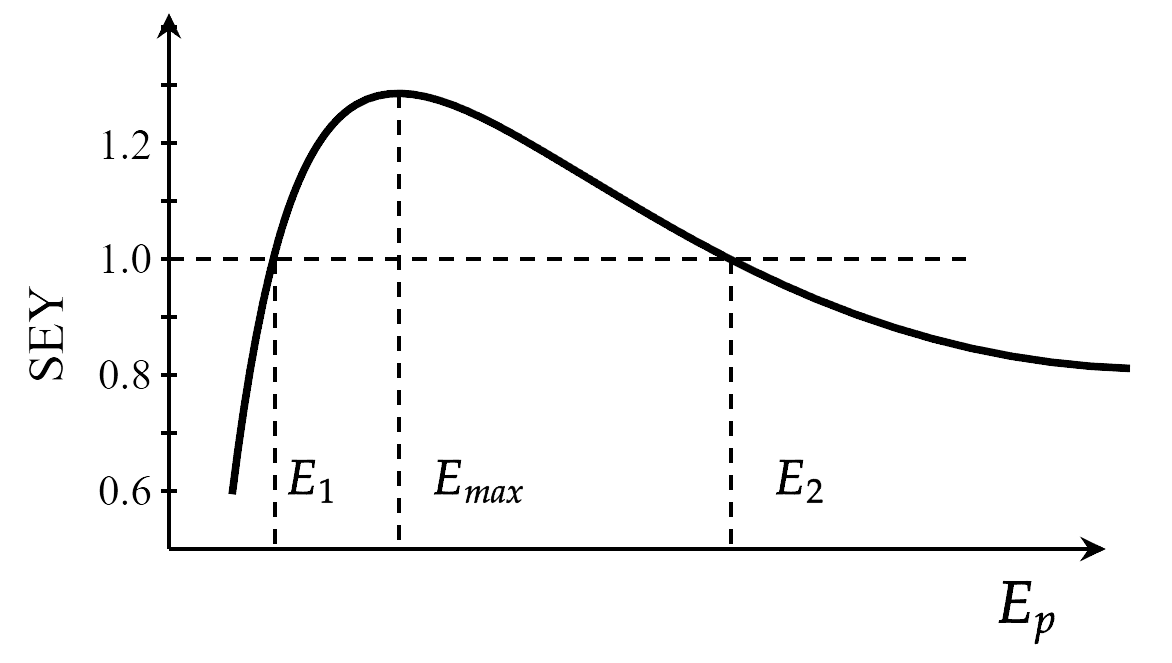
\includegraphics[width=\textwidth]{pic/chapter2/二次电子发射曲线.png}
    \caption{金属的典型的二次电子发射曲线}
    \label{fig:SEY_EP}
\end{figure}

这个曲线在三个特征点处有着各自对应的物理意义,图中的$E_1$表示着入射电子轰击能量从0开始逐渐增大的过程中,SEY首次等于1时的入射电子能量值;$E_{max}$对应着SEY到达最大值时候初始电子能量的值。根据之前分析,再增大入射电子能量SEY值反而会回落,此时的$E_2$值便表示着随着入射能量的继续增大,在SEY值到达最大值之后,再次回落到1时候的入射能量$E_p$的值。

为了准确的描述与预测SEY随着入射能量的变化而产生的变化,有必要建立相关数学物理模型。相关的描述模型有很多,比较有代表性的的模型便是Furman\citing{furman_2002_model}模型和Vaughan\citing{vaughan_1988_multipactor,vaughan_1989_newformula}模型。由于Furman模型针对入射电子轰击到固体材料表面之后的物理过程进行了诸如散射或者被材料吸收等的分类,但是实际上进行实际的测量实验时针对详细的物理过程难以进行实际的观察。为了使用Furman来提高实际拟合精度所付出的代价要远大于直接使用Vaughan模型进行数值拟合。故本文研究的主要模型是Vaughan模型,本文之下将要详细介绍的也是此模型。Vaughan模型是一种唯象模型,其只针对二次电子发射现象进行数据拟合,并未从中提取出更为严谨的物理机理。但是其数据拟合方便并且也比较精准,至今仍在研究二次电子发射现象过程中被广泛使用。

描述SEY的Vaughan模型中的计算公式为:

\begin{equation}\label{eq:SEY_Vaughan}
    \frac{\delta(\theta)}{\delta_{\max}(\theta)} = 
    \begin{cases} 
    \left( \varepsilon e^{1 - \varepsilon} \right)^{0.56} & \text{if } \varepsilon \leq 1 \\
    \left( \varepsilon e^{1 - \varepsilon} \right)^{0.25} & \text{if } 1 < \varepsilon \leq 3.6 \\
    \frac{1.125}{\varepsilon^{0.35}} & \text{if } \varepsilon > 3.6
    \end{cases}
\end{equation}
其中,
$$
\varepsilon = \frac{E_p - E_t}{E_{\max}(\theta) - E_t}
$$

$$
\delta_{\max}(\theta) = \delta_{\max}(0) \left( 1 + k_s \frac{\theta^2}{2\pi} \right)
$$

$$
E_{\max}(\theta) = E_{\max}(0) \left( 1 + k_s \frac{\theta^2}{2\pi} \right)
$$

以上公式中,$E_p$为入射电子能量,$\theta$为入射电子角度,$\delta_{max}$为SEY的最大值,$E_{max}$为$\delta_{max}$所对应的入射电子能量,$E_t$为入射电子截止能量,$k_s$为表面光滑度因子。

为了减小电子倍增现象对器件造成的影响,可以在了解影响材料的SEY影响原因之后,针对性的对器件的结构进行改造进而减小电子倍增现象的产生。例如,不同的固体材料的SEY值不同,可以选择低SEY材料对材料表面进行处理或者使用直接使用材料\citing{ren_2020_multipactor_simulation}对器件进行填充;其次是确保器件的表面光整度以及减少加工过程中\citing{li_2021_novel_multipactor}产生的缝隙,如果材料的表面较为粗糙或者有加工缝隙,会导致斜射到材料表面的概率增加,从而导致产生二次电子倍增现象的概率增加。除了上述所提到的主要影响原因之外,有时候SEY还会遇到诸如材料在空气中受到氧化进而产生性质变化,或者大气压的变化等原因产生影响。
\subsection{由于热应力引起的损毁}

\chapter{6-11GHz 宽频带脊波导窗的设计}
\section{传统结构盒型窗的局限性}
[使用适当的理论计算,计算出t-l之间的关系进行配图]
在前面\ref{sec:PillBoxTheory}中提到的传统结构的微波窗在许多方面上存在局限性。首先从加工层面来说,因为圆形窗片的半径与圆柱形波导的直径相同,如果想要固定介质窗片,那么就必须从侧面对窗片进行焊接。侧面焊接的气密性与窗片的厚度有关,如果窗片太薄,那么在焊接的过程中就会出现不稳定性,并且窗片的机械强度也会受到影响,过薄的窗片很容易出现打火击穿或者内外压差进而碎裂的情况。观察不等式\ref{eq:Delta}并且结合等式\ref{eq:B_d}可以发现,想要特征方程\ref{eq:B-C-simplify2}有解,那么对于窗片的厚度$t$的取值范围有:
\begin{equation}\label{eq:t_constraints}
    0 < t < \frac{\sqrt{\frac{1}{k^2}+4k^2(1+B_{T}^2)^2-2(1-2B_{T}^2)}}{(\varepsilon_{d}-1)(\omega / c)(\lambda_{gc} / \lambda)}
\end{equation}
传统盒型窗的特征方程说明了,为了确保盒型窗能够正常建造,窗片的厚度$t$必须小于一个阈值,过厚的窗片不能使用实现传统盒型窗的匹配方法进行匹配。

其次,根据之前\ref{sec:PillBoxTheory}中提到的,传统模式的盒型窗的单侧匹配电长度不能低于0.1倍电长度,因为盒型窗需要两端匹配段,那么可以得到盒型窗匹配段连带窗片部分的电长度不会低于0.2倍电长度。这一点难以保证盒型窗在实际进行匹配时候的结构紧凑性。

最后,根据文献\cite{huxiongli_bandwidth_pill},传统意义上的盒型窗的相对带宽一般会在15\% 到20\% 之间。如果想要进一步的提升盒型窗的带宽,只能对其结构进行相应的改进,例如将窗片的厚度进行进一步的削减,这一步骤势必会进一步的影响窗片的机械结构强度与气密性。
\section{宽带宽波导窗概述}
现阶段常用的几种宽带宽微波窗的实现方案可以被总结为如下几点,这些方案主要用于改进微波窗与输能波导之间的匹配部分,使得窗片能够在更宽的范围内实现匹配的特点。

在论文\cite{cook_broadband_2013_gradually}中,作者使用渐变段实现了从矩形波导的$TE_{10}$到圆波导的$TE_{11}$模式的渐变过渡,使得窗片的匹配带宽得到增宽。经过作者的调整,实现了材料为氧化铍的窗片,在212-225GHz 的范围内达到$S_{11}$的匹配程度。渐变过渡的优点是较为容易进行设计,并且只要确定前后段的形状后便能使用现有的如小反射理论等理论进行设计。但是缺点是,为了实现这种渐变的过渡段,需要牺牲器件的紧凑性,器件的匹配部分在纵向长度上来说显得较为冗长。

另外一种增加窗片带宽的方案是使用布儒斯特窗\citing{sharan_broadening_2020},将窗片进行倾斜[布儒斯特窗的工作原理是什么来着?为什么相对于传统窗片布儒斯特窗的频带更宽?]。

原作者在这个方案中,使用了使用化学气相沉积法得到的钻石窗片,得到了在111.6-165.7GHz 范围内的回旋管中的十个不同模式均有不错的匹配效果的结果。布儒斯特窗相比于传统的盒型窗,不需要进行匹配段的设计,窗片的匹配与波导浑然一体。但是布儒斯特角的窗片为倾斜焊接的椭圆形窗片,并且在装具焊接过程中部分窗片外露于波导之外。这使得布儒斯特窗在应力方面,相比于传统的圆形窗片更大。并且在加工焊接方面,由于要同时控制窗片的倾斜角与椭圆窗片长轴的朝向,对于装具焊接加工的精度要求更高。

此外还有一种增加窗片带宽的方案是多层窗。[物理原理是什么?]

多层窗是一个包罗范围较为广泛的解决方案,其中包含了窗片使用多种不同相对介电常数堆叠的方案\citing{wang_broadband_window_2017, donaldson_multilayer_2013, li_meta_2025},也包括了窗片在纵向方向上进行阶梯状的形变进而实现匹配的方案\citing{liu_multilayer_broadband_2021,chen_multilayer_broadband_2020},还包括了窗片的匹配段进行紧凑型多层阶梯过渡的方案\citing{ali_multilayer_broadband_2020}。大部分都可以被等效为不同的相对介电常数堆叠的方案,它们最多可以达到49\% 的相对带宽,并且大部分的设计都非常紧凑,节省了器件在纵向上的匹配所需的长度空间。但是由于需要考量不同层数的相对介电常数,以及调控这些层数的纵向长度,这使得相比于传统的窗,多层窗的设计更加繁琐。并且多层窗在设计完毕之后的进一步的加工方面,多层窗片层级之间可能存在空隙使得匹配状况变差。并且上述提到的多层或者异形窗片在最终的焊接过程中,熔融焊料易渗入界面缝隙。装配工序中,残留焊料产生的应力使多层或者异形窗发生翘曲位移,致使实际装配参数偏离理论设计值,影响微波窗整体性能\citing{dajunzhao_capasity_2023}。

\section{输入窗的相关研究}
为了解决盒型窗带宽与机械结构之间的矛盾,以及常见的宽带宽窗片解决方案造成的较难以焊接加工或者设计的相关问题。现在对原先的盒型窗片的结构进行进一步的改良,获得一种新型的以脊波导为传输波导,并且以圆形窗片为输入窗片,以圆角矩形为脊波导到窗片之间的过渡段的新型的宽带宽窗。
\subsection{新型脊波导窗的设计}
本次设计的波导窗必须满足以下设计要求:
\begin{enumerate}
    \item 窗片在6-11GHz之内,满足$S_{11}<-20dB$的匹配要求(相对带宽58\%)。
    \item 结构结构紧凑,方便器件的小型化。
    \item 窗片几何结构较为简单,方便后续的加工与焊接。
\end{enumerate}

由于脊波导相比于同等频段的矩形波导结构更加紧凑,主模带宽更宽,以及双脊波导的功率容量比单脊波导的功率容量更大。结合小节\ref{subsec:DoubleRidgeTheory}里面的关于双脊波导理论研究,现在初步确定双脊波导的几何参数参数如下:$a=20mm, b=10mm, d=5mm, s=4mm $,具体的脊波导横截面如图\ref{fig:6-11GHzDRW}所示:
\begin{figure}[!htb]
    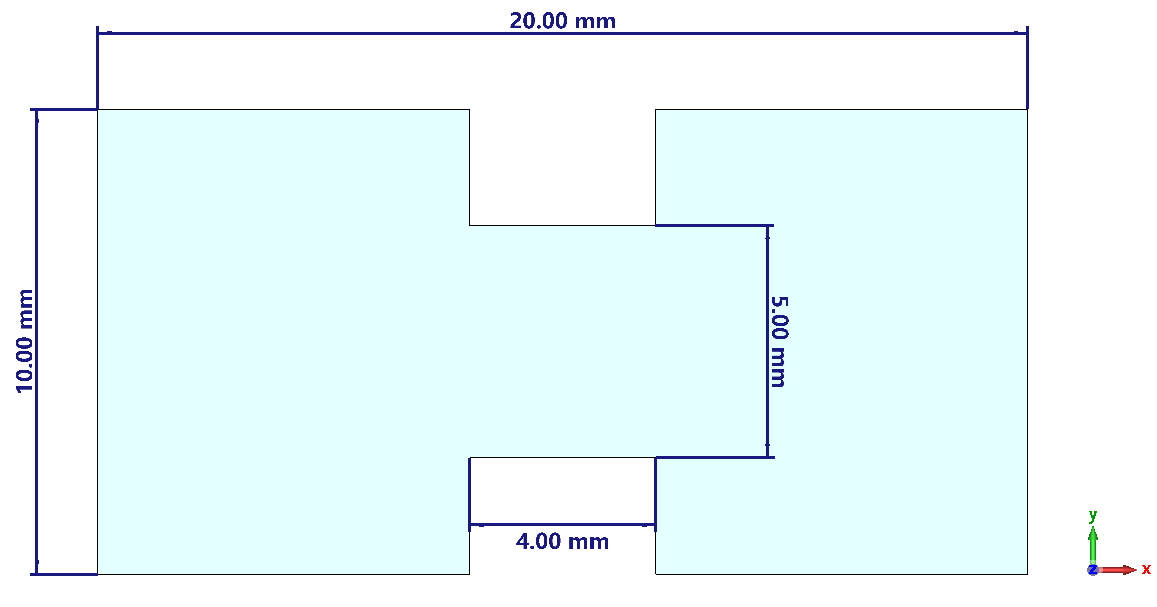
\includegraphics[width=0.7\linewidth]{pic/chapter3/6-11GHzDRW.png}
    \caption[short catption 1]{输入窗脊波导几何参数选取}
    \label{fig:6-11GHzDRW}
\end{figure}

很明显,这个脊波导的几何参数满足式子\ref{eq:DRW_constraints}的限制条件,此时可以通过简化式子\ref{eq:DRW_closed}计算双脊波导的截止频率进行计算,得到的计算结果为$f_c=5.85GHz$。此时截止频率小于所需带宽的下限,表明此时选取的脊波导几何参数满足要求。现在使用CST对脊波导的真实截止频率以及直通情况下的S参数进行仿真,得到如图\ref{fig:脊波导初步仿真}的结果。根据图\ref{fig:脊波导初步仿真} (a)结果显示,脊波导的截止频率为$f_c=5.84GHz$,与式子\ref{eq:DRW_closed}的计算结果基本一致。根据图\ref{fig:脊波导初步仿真} (b)显示,此时的双脊波导在要求的频段6-11GHz之内$S_{11}<25dB$,满足匹配要求。

\begin{figure}[!htb]
    \small
    \centering
    \begin{tabular}{@{\ }c@{\ }c}
        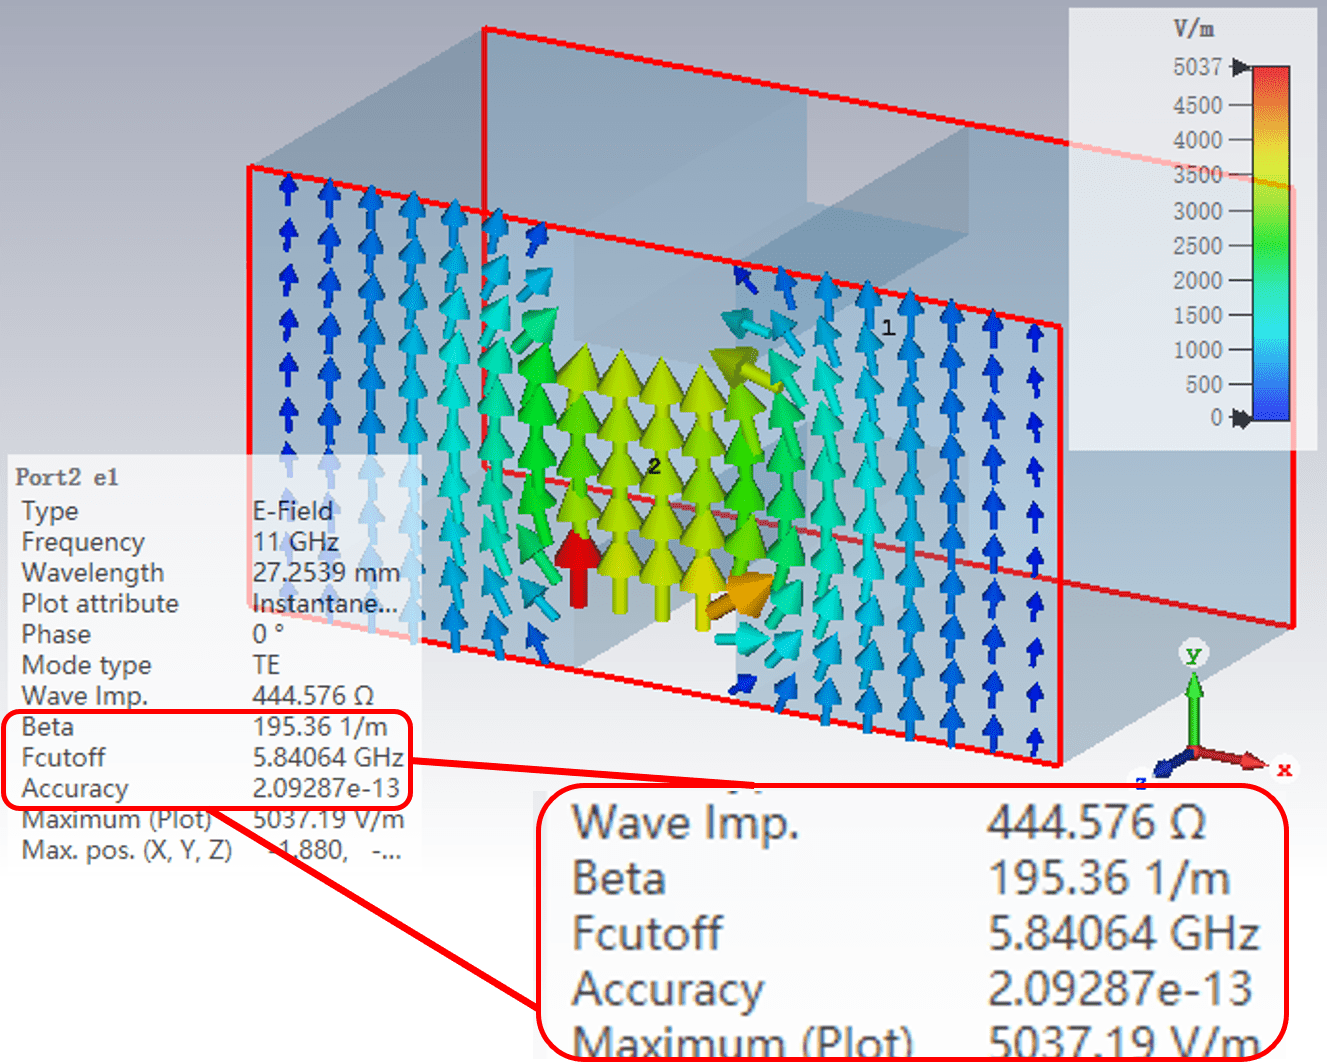
\includegraphics[width=0.45\textwidth]{pic/chapter3/脊波导初步仿真.png} & 
        \hspace{5pt}
        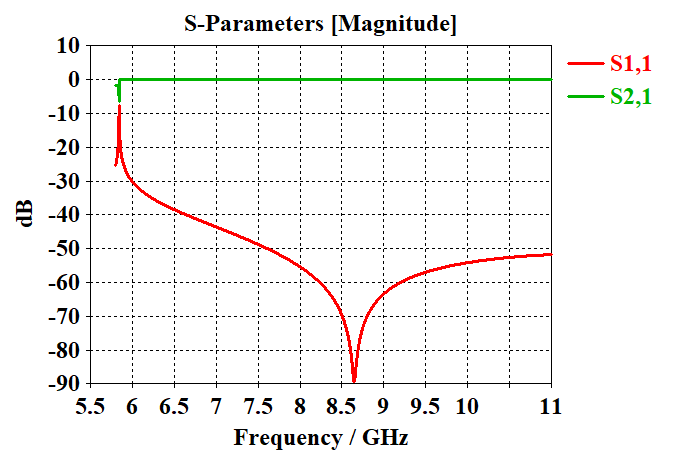
\includegraphics[width=0.45\textwidth]{pic/chapter3/输入窗脊波导S曲线.png}     \\
        \mbox{\small (a)脊波导截止频率仿真}                                                                               & 
        \mbox{\small (b)脊波导S曲线仿真}                                                                                  \\
    \end{tabular}
    \caption{脊波导初步仿真}
    \label{fig:脊波导初步仿真}
\end{figure}

接下来选取脊波导圆形窗片的材料,根据文章\cite{han_sapphire_2011}里面对窗片材料的论述,蓝宝石的特性包括低介电损耗和高机械强度,使其能够制造出0.1毫米厚的精细层而不会因为管内外压差而产生破损;由于它是致密无孔的晶体材料,内部结构均匀,所以在高功率操作环境下不易发生熔解破坏。此外,它还能应对焊接和真空脱气过程中的高温,当实现大规模生产时,成本控制良好,且环保方面的问题较少。因为蓝宝石的上述优点,本文选取蓝宝石作为窗片的材料。根据材料\cite{thumm_2020_State}所示,将蓝宝石的相对电介质常数设定为$\varepsilon_r=9.4$,损耗角正切被设定为$\tan \delta = 0.0004$。

经过计算仿真,最终确定脊波导窗片的整体结构为图\ref{fig:脊波导窗的整体结构}所示。
\begin{figure}[!htb]
    \centering
    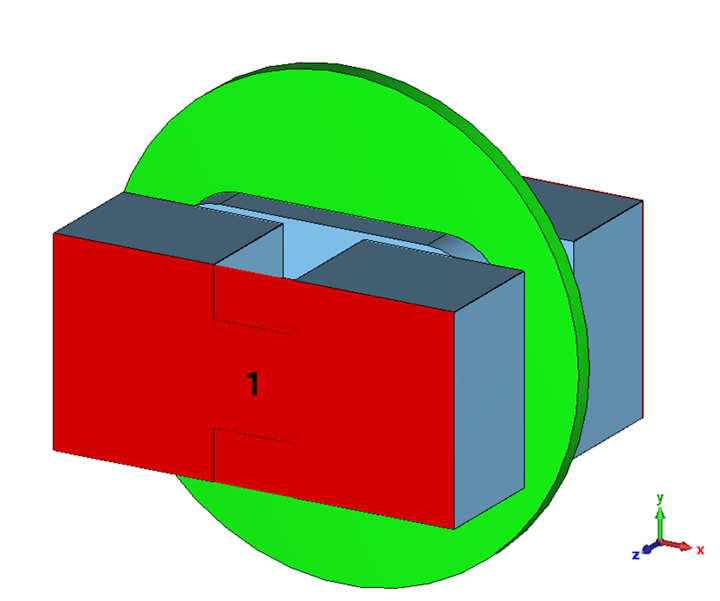
\includegraphics[width=0.45\linewidth]{pic/chapter3/输入窗的总体视图.png}
    \caption{脊波导窗的整体结构}
    \label{fig:脊波导窗的整体结构}
\end{figure}

为了方便设计加工与焊接,窗片被设置为圆形窗片。为了减少匹配段的长度,窗片与脊波导之间的过渡部分被设计为倒圆角的矩形过渡段。其中对过渡部分倒圆角不仅是为了降低过渡段的最大场强,提升窗片的功率容量,防止窗片被击穿;另一方面也方便了之后对过渡段部分的加工。

各个部分的详细尺寸被记载于图\ref{fig:窗片与过渡段的尺寸}中。其中\ref{fig:窗片与过渡段的尺寸} (a) 展示了窗片的直径为22.98mm。图片\ref{fig:窗片与过渡段的尺寸} (b)展示了圆窗片与脊波导之间的圆角矩形过渡段的具体尺寸,其长边为16.03mm,短边为10.61mm,四个角均倒圆角,倒圆角的半径为2.85mm。结构具体的纵向长度如图\ref{fig:窗片与过渡段的尺寸} (c)所示,圆角矩形过渡段的纵向长度为1.69mm,窗片的厚度为0.91mm。

\begin{figure}[!htbp]
    \small
    \centering
    \begin{tabular}{@{\ }c@{\ }c}
        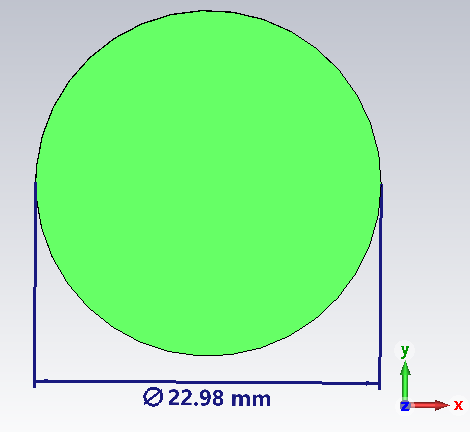
\includegraphics[width=0.25\textwidth]{pic/chapter3/圆形窗片视图.png} & 
        \hspace{5pt}
        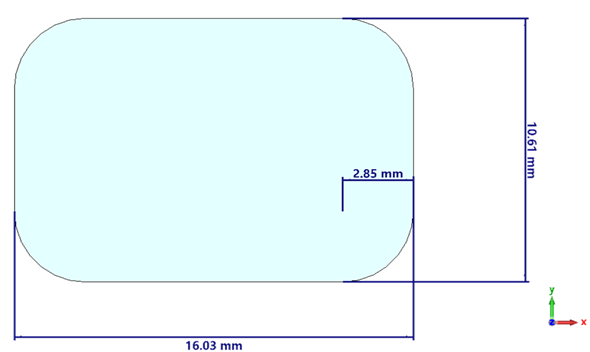
\includegraphics[width=0.45\textwidth]{pic/chapter3/圆角矩形视图.png}     \\
        \mbox{\small (a)圆形窗片视图}                                                                               & 
        \mbox{\small (b)圆角矩形视图}                                                                                  \\
    \end{tabular}
    \\[6bp]
    \begin{subfigure}[t]{0.75\linewidth}
        \setcounter{subfigure}{2}
        \centering
        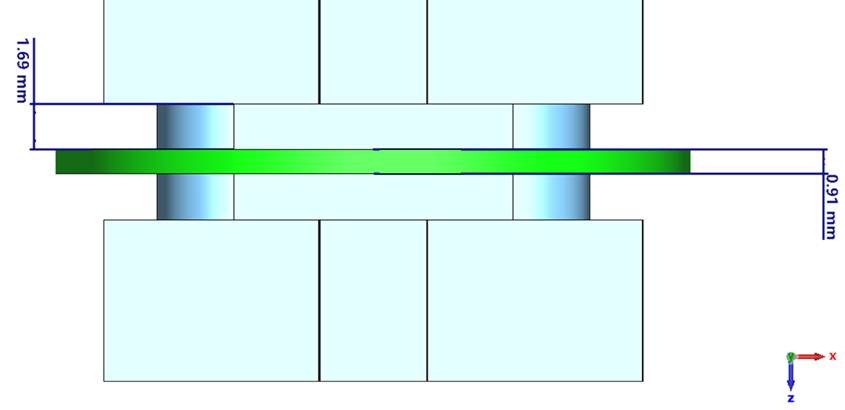
\includegraphics[scale=0.21]{pic/chapter3/纵向长度视图.png}
        \caption{纵向长度}
        \label{subfig:纵向长度视图}
    \end{subfigure}
    \caption{窗片与过渡段的尺寸}
    \label{fig:窗片与过渡段的尺寸}
\end{figure}


此时对脊波导窗的过渡段部分电长度进行分析,并与传统盒型窗进行对比。根据上文的分析,为了满足盒型窗窗片两侧过渡部分能够被等效为传输线的物理模型这一目的,传统盒型窗的匹配段部分不得小于0.1倍电长度。如果不满足这一要求就会因为无法被等效为传输线模型进而导致设计的匹配点出现频偏。此时新型盒型窗的过渡段可以被视作工作在$TE_{01}$下的长边为16.03mm,短边为10.61mm矩形波导,计算其在$10GHz$的工作波长为$\lambda_{gRec}=\lambda / \sqrt{1-(\lambda / \lambda_c)^2}=85.06mm$,匹配部分的电长度小于0.1倍电长度,相比于传统盒型窗的匹配部分的电长度更短,故新型窗片的匹配部分结构更加紧凑。

此时对原先参数的脊波导窗在CST里面进行建模,并且使用频域求解器在匹配频段内进行仿真,计算得到窗片的S参数如图\ref{fig:输入窗的S参数}所示:

\begin{figure}[!htb]
    \centering
    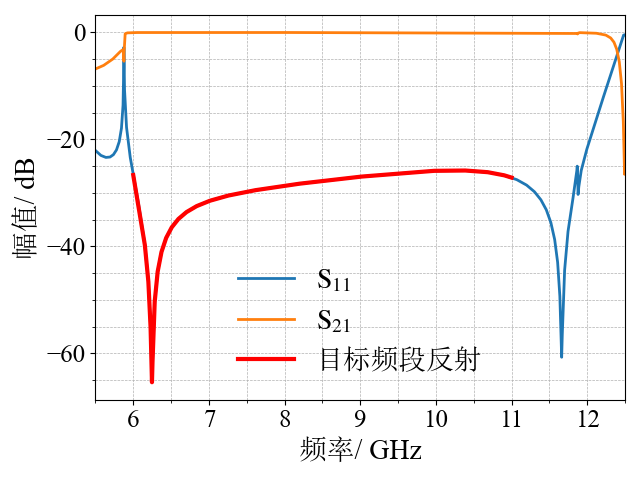
\includegraphics[width=0.5\linewidth]{pic/chapter3/脊波导窗S参数.png}
    \caption{输入窗的S参数}
    \label{fig:输入窗的S参数}
\end{figure}
对窗片的S参数进行考察,发现其反射系数$S_{11}$在要求的频段6-11GHz之内小于-20dB,满足匹配要求。此时结合图片可以得到满足反射系数$S_{11}<-20$的频带范围为6-11.5GHz,此时计算其相对带宽为62.9\%。
\subsection{脊波导窗的参数敏感度分析}
ERRORFIX。
\subsection{计算脊波导窗功率容量}
为了探究输入窗的适用范围,有必要对脊波导窗的功率容量进行分析。微波窗通常在电场强度最强处出现击穿,并且在扫参时候发现,在同一匹配频段内,低频点的电场强度更强。根据这些结论,现在对脊波导窗的在低频点(6GHz)处的电场场强进行仿真,得到如图\ref{fig:脊波导窗低频点场强仿真}所示的结果:
\begin{figure}[!htb]
    \centering
    
\includegraphics[width=0.25\linewidth]{pic/ERROR.jpg}
    \caption{脊波导窗6GHz场强仿真}
    \label{fig:脊波导窗低频点场强仿真}
\end{figure}

为了方便进一步地分析,需要找到最大电长场强所在位置,使用CST进行仿真之后可以得到其最大场强出现在ERROR,具体位置如\ref{fig:脊波导窗低频点场强仿真}所示:
\begin{figure}[!htb]
    \centering
    
\includegraphics[width=0.2\linewidth]{pic/ERROR.jpg}
    \caption{脊波导窗6GHz场强仿真}
    \label{fig:脊波导窗6GHz场强仿真}
\end{figure}

完成最大场强所在位置之后,可以开始对脊波导窗功率容量进行进一步的分析。为了确保结果的准确性,本文采用了两种不同的仿真方式进行对照。
\subsubsection{使用最大场强法计算脊波导窗的功率容量}
最大场强法主要是通过对端口的输入功率进行扫参,根据经验值,室温常压下的空气的击穿场强是30kV/cm。故在进行仿真的时候,如果瞬时电场的最大场强值达到30kV/cm的空气击穿场强时便被视为击穿。但是在实际的窗片加工的过程中,窗片的实际功率容量并不全与这个方法所计算出来的功率容量相一致,实际情况下由于环境的不同,空气的击穿场强也会随着产生变化。并且窗片损毁的原因也不一定完全与最大场强相关,有可能由于电子倍增现象在介质表面存积电子进而产生闪络击穿现象。故此方法得到的功率容量的值仅供参考,在实际应用过程中需要针对最大场强法进行计算的功率容量进行修正。

此时在低频点(6GHz) 处设定电场监视器,并且使用后处理模板提取电场监视器的电场场强的最大值作为跟根据仿真结果\ref{fig:输入窗最大场强结果}显示,在馈入端口的功率到达7.5kW的时候,窗片内的最大场强达到30kV/cm。此时的窗片的功率容量应该在7.5kW左右。这个功率容量对于输入窗口来说已经足够。
\begin{figure}[!htb]
    \centering
    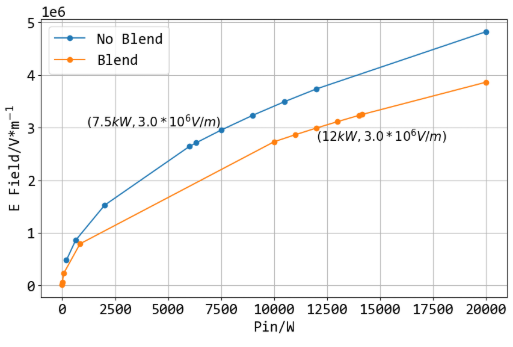
\includegraphics[width=0.5\linewidth]{pic/chapter3/脊波导最大场强.png}
    \caption{输入窗最大场强结果}
    \label{fig:输入窗最大场强结果}
\end{figure}

\subsubsection{使用电子倍增计算脊波导窗的功率容量}
正如前面小节\ref{sec:电子倍增现象理论}中所说,电子倍增现象是影响真空器件在太空中的功率容量的重要原因。为了更加完全验证器件的功率容量,除了前面的最大场强分析法,有必要使用二次电子倍增理论对器件的功率容量进行进一步的分析。

前面已经使用CST针对器件的S参数进行了仿真并且已经验明原先的器件的S参数符合设计要求,本次将使用CST中的SPARK3D模块进行先验仿真,并使用PIC模块对原先的器件进行基于二次电子倍增的详细功率容量仿真。

由于关于二次电子产额和入射电子能量相关曲线有许多种不同的测量方法,每种测量方法之间的结果与精度\citing{guanghuimiao_2018_measurement}相差较大,并且不同的二次电子发射曲线所带来的结果也不尽相同,故本文在引用二次电子发射曲线时尽量从多篇文章中找到曲线并且对参数进行综合考量后再进行分析。

首先根据文献\cite{valizadeh_2014_wja}能获得关于在Vaughan模型中中入射电子能量从80到1000电子伏特时候的二次电子发射曲线,的铜的二次电子发射曲线的关键参数分别为$\delta_{max}=1.9, E_{max}=300 eV$;在文章\cite{bojko_2020_see}中测量了入射电子能量从60到3000电子伏特的铜的二次电子发射曲线,其关键参数为$\delta_{max}=1.6, E_{max}=352 eV$;文章\cite{jianweifang_lizi_2023}中测量了入射电子能量从50到1000电子伏特的铜的二次电子发射曲线,其关键参数为$\delta_{max}=1.76, E_{max}=250 eV$。从这些论文中综合他们所测量的二次电子发射曲线,可以得到使用Vaughan模型的无氧铜的二次电子发射曲线中的关键值为:$\delta_{max}=1.9, E_{max}=300 eV$,并且设置CST中的二次电子发射曲线的入射电子能量区间为50到1000电子伏特,入射方式为垂直入射,其余参数保持默认。

此时根据文献\cite{suharyanto_2006_secondary}测量了入射电子能量从0.5-5keV的蓝宝石二次电子发射系数,此时相关的关键参数为$\delta_{max}=7.91, E_{max}=0.99keV$;文献\cite{chvyreva_2014_experimental}展示了蓝宝石的二次电子发射曲线关键参数为$\delta_{max}=7.8, E_{max}=0.65keV$。本文后续使用的参数为$\delta_{max}=7.91, E_{max}=0.65keV$,CST中设置二次电子发射曲线的入射电子能量区间为50到5000电子伏特,入射方式为垂直入射,其余参数保持默认。本文后续将使用这些文献中所展示的关键参数,结合前文中所示的Vaughan模型\ref{eq:SEY_Vaughan}对器件的二次电子发射情况进行仿真,设置完成后的曲线如图\ref{fig:X波段材料二次电子发射特性}所示。
\begin{figure}[!htb]
    \small
    \centering
    \begin{tabular}{@{\ }c@{\ }c}
        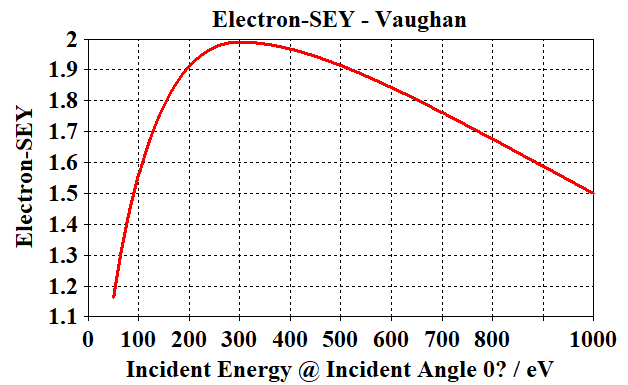
\includegraphics[width=0.4\textwidth]{pic/chapter3/铜的SEY.png} & 
        \hspace{5pt}
        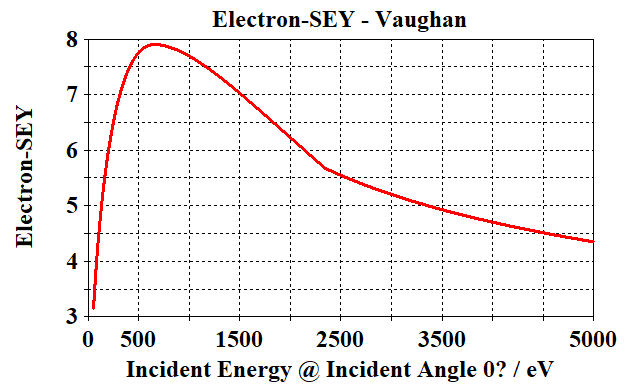
\includegraphics[width=0.4\textwidth]{pic/chapter3/蓝宝石的SEY.png}     \\
        \mbox{\small (a)铜二次电子发射曲线}                                                                               & 
        \mbox{\small (b)蓝宝石二次电子发射曲线}                                                                                  \\
    \end{tabular}
    \caption{Vaughan模型下材料的二次电子发射特性}
    \label{fig:X波段材料二次电子发射特性}
\end{figure}

为了方便进行二次电子发射曲线的设置,需要将窗片使用无氧铜外壳进行包覆。为了验证背景材料更改为无氧铜之后是否会对窗片本身的电磁特性产生影响,现在将背景材料更改为无氧铜进行关于S曲线的仿真。此时无氧铜的电导率被设置为$\sigma = 5.8 \times 10^7 S/m$。仿真结果在图\ref{fig:X无氧铜背景}中被展示,结果表明背景材料被更改为无氧铜并没有对S曲线产生太大的影响,可以使用无氧铜作为原先窗片的外壳进而进行后续的仿真。
\begin{figure}[!htb]
    \centering
    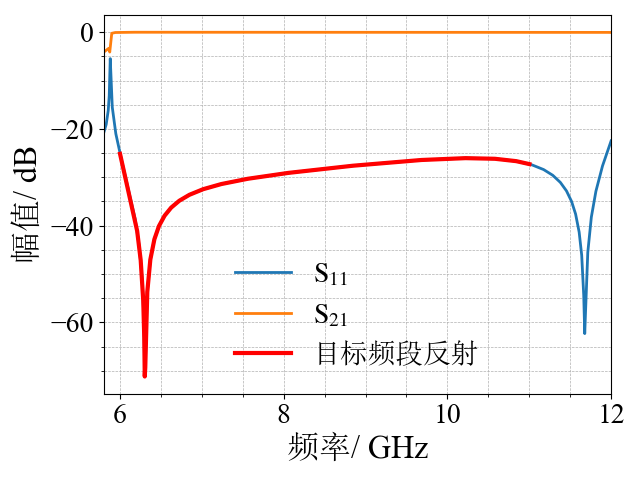
\includegraphics[width=0.5\linewidth]{pic/chapter3/X脊波导窗无氧铜.png}
    \caption{X波段脊波导无氧铜背景下的S曲线}
    \label{fig:X无氧铜背景}
\end{figure}

为了方便后续的二次电子仿真,有必要使用CST中专门进行电子倍增仿真的Spark3D模块进行预先仿真。Spark3D模块不仅可以看出原先器件中哪些地方的电场强度更强,也可以根据已经设定好的二次电子发射曲线,来进行初步的功率容量仿真。这些预先的结果都为了进一步的使用CST进行PIC的仿真提供了方便,有助于减少进一步仿真中关于功率的迭代次数。首先将CST中频域求解器已经仿真好的电场磁场强度结果导出成Spark3D模块可以使用的$.f3e$格式,并且导入Spark3D,材料相关的二次电子发射曲线参考之前所找到的材料和\ref{fig:X波段材料二次电子发射特性},尽量做到跟PIC求解器中的二次电子发射曲线参数一致。Spark3D中的初始轰击电子的位置是随机的,其在每次仿真过程中并无法得到完全相同的功率容量。为了确保仿真结果的真实性,需要适当的增加Spark3D中的初始电子数目需要增加,本次在Spark3D中放置初始电子数目为800。

图片\ref{fig:X波段Spark3D中的电场}展示了X频段脊波导窗中电场分布,参考文献\cite{guobao_2019_intera}中关于电场强度的说法,此时可以得知电场场强最强的部分是脊波导的脊,以及脊波导和窗中间的过渡部分的圆角矩形部分。由于器件工作在低频点时更容易被击穿,故此时在Spark3D中的激励信号被设置为6GHz的连续波。
\begin{figure}[!htb]
    \centering
    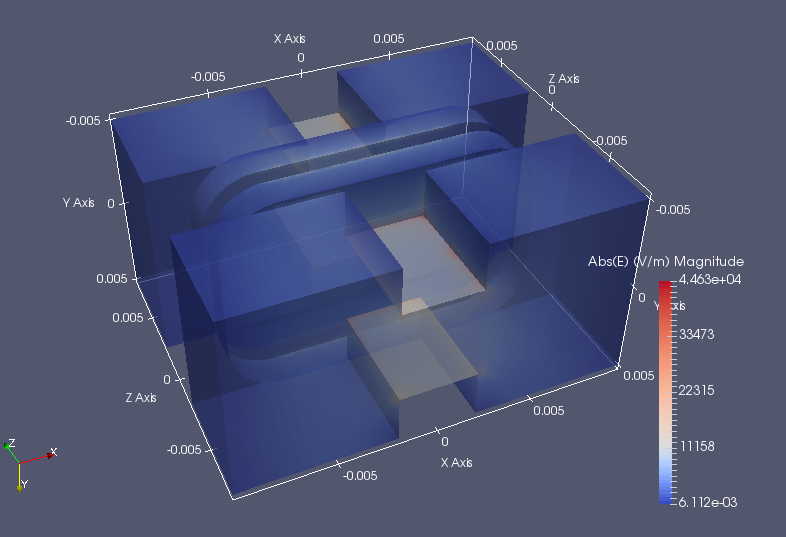
\includegraphics[width=0.5\linewidth]{pic/chapter3/X波段Spark3D中的电场.png}
    \caption{X波段脊波导Spark3D中的电场}
    \label{fig:X波段Spark3D中的电场}
\end{figure}

结合以上分析与初始设定,此时使用Spark3D初步仿真得到窗片的功率容量为REFERROR,具体仿真结果如图\ref{fig:X波段Spark3D中的功率}所示。
\begin{figure}[!htb]
    \centering
    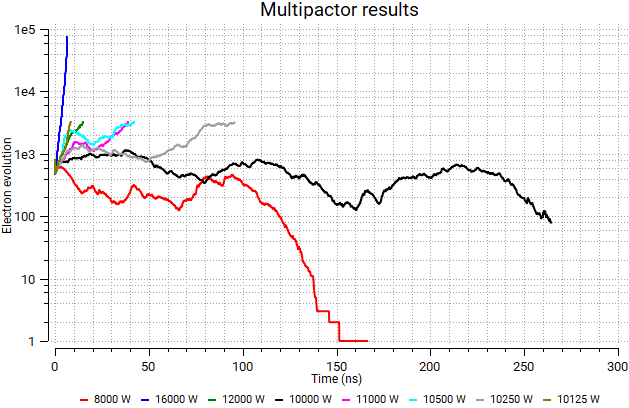
\includegraphics[width=0.5\linewidth]{pic/chapter3/X波段Spark3D中的功率.png}
    \caption{X波段脊波导Spark3D中计算的功率}
    \label{fig:X波段Spark3D中的功率}
\end{figure}
不同与SPARK3D的材料设定,CST的PIC求解器不能设置背景材料的二次电子发射系数,此时需要对窗片套上一定厚度的外壳后进行进一步的二次电子仿真。为了方便建模,将原先的真空仿真模型外侧套上了一个宽和高比最大模型外侧还要大2mm的立方体外壳,套上外壳之后的窗整体如图\ref{fig:X无氧铜外壳}所示。
\begin{figure}[!htb]
    \centering
    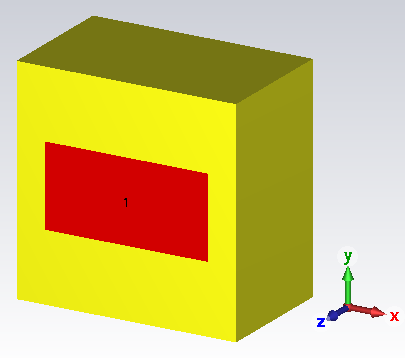
\includegraphics[width=0.4\linewidth]{pic/chapter3/X脊波导窗无氧铜外壳.png}
    \caption{X波段脊波导无氧铜外壳下的S曲线}
    \label{fig:X无氧铜外壳}
\end{figure}

此时CST的默认激励端口的信号为脉冲激励,并不符合实际上使用时候的输入信号模型,应该改为连续波激励。本次仿真所使用的是连续正弦信号激励,由于在实际使用的过程中,在低频更容易被击穿,故本次连续波激励信号的频率被设定为原规定频域(6-10 GHz)的最低频点6 GHz处。此时的连续波激励信号如图\ref{fig:X波导窗连续波激励信号}所示。经过初步的CST PIC仿真与设置粒子轨迹监视器发现,在正常工作功率范围内的连续波信号的激励情况下初始电子的消失时间约为90ns。根据以前的实验经验,连续波的激励时间和总仿真时间应该不低于这个时间的两倍,故连续波的正常激励时间和总仿真时间被设定为200ns。
\begin{figure}[!htb]
    \centering
    
\includegraphics[width=0.5\linewidth]{pic/ERROR.jpg}
    \caption{X波段脊波导窗连续波激励信号}
    \label{fig:X波导窗连续波激励信号}
\end{figure}

具体的仿真流程中,经常使用在器件中放置一定数目的电子作为初始的种子粒子,然后再使用电场来驱动这些粒子对器件的表面进行轰击,进而通过观察此时的初始粒子数目随着时间的的变化情况来判断器件是否被击穿。具体的放置种子粒子的密度以及判断器件的击穿标准在不同的文章中也不尽相同,但是可以选取几篇文章作为相应的参考。根据文章\cite{li_2021_novel_multipactor}中的描述,如果器件中的电子数目在信号驱动的情况下呈现出指数函数式的增长,那么就被视为期间会因为二次电子发射而击穿,如果器件中电子的数目随着信号的激励呈现出持续下降的趋势就被视为没有击穿。关于具体的种子粒子的放置,文献\cite{gonzalez_2015_experimental}在仿真同轴波导的时候,初始的种子粒子数目为500,判断其被击穿的条件为仿真过程中电子总数大于$10^4$;文献\cite{gonzalez_2016_multipactor}在仿真同轴波导时,初始的电子数目为$10^{12}$个,等效的电子密度为$4.83 \times 10^{17} m^{-3}$,由于激励信号并非使用正弦函数,故击穿的条件被设定为“20间隙击穿”法则;文献\cite{you_2015_highly}中在脊波导器件的最窄处填充了8000个电子,并且也是因为电子数目在正弦信号驱动情况下呈现指数增长才被视为击穿,如果是持续下降的电子趋势就被视为没有击穿。

综合上述文献的描述与仿真速度精度的要求,本文决定在填充初始电子时候选择电场强度最强的部分进行立方体形状的麦克斯韦能量分布的粒子源填充,而不是所有空白区域全部都进行相同的能量的电子填充,并且填充的电子的密度不低于$10^9 m^{-1}$。如果器件中电子的数目随着信号的激励呈现出持续下降的趋势就被视为没有击穿;如果总粒子数目呈现出指数函数式的增长,那么在总粒子数目达到$5 \times 10^5$个之后便被视为击穿。结合之前在Spark3D中的预仿真,还有一种电子数量没有明显增长但是也没有明显减小的情况,此时其二次电子产生和电子的被吸收速率相近,在电子数目中达到了动态平衡,这种情况依然对器件有击穿的风险,故也被视为击穿。根据Spark3D和之前图\ref{fig:脊波导窗低频点场强仿真}中的预先仿真,可以得知此时的电场场强最强的部分是脊波导的脊,以及脊波导和窗中间的过渡部分的圆角矩形部分,具体的填充区域示意图可见\ref{fig:X粒子填充区域}中所示。
\begin{figure}[!htb]
    \centering
    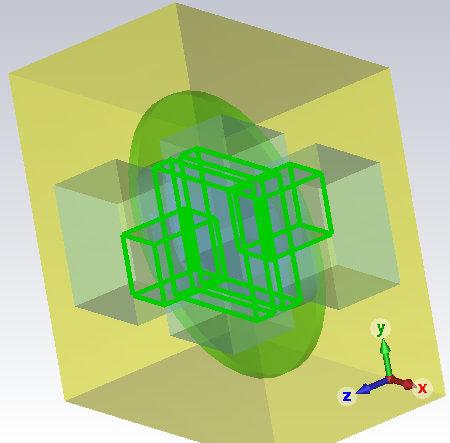
\includegraphics[width=0.5\linewidth]{pic/chapter3/粒子填充区域斜视图.png}
    \caption{X波段脊波导窗粒子填充区域}
    \label{fig:X粒子填充区域}
\end{figure}

在进行好了材料二次电子发射曲线、正弦连续波激励信号、初始麦克斯韦能量分布的电子的粒子填充和明确了因为电子倍增现象而击穿的规则之后,便可以对器件进行基于电子倍增现象的功率容量的仿真。仿真得到的整体粒子数目随着馈入连续波时间的变化而产生的变化的曲线被展示与图片\ref{fig:X波段脊波导窗基于电子倍增现象的功率容量仿真}中。从图片中可以看到,在馈入能量达到14.8kW之前,器件中粒子数目随着时间的变化呈现为持续下降的趋势;在能量到达15kW时电子数目达到动态平衡;但是在馈入连续波能量达到15.3kW之后,粒子数目呈现出指数式的增长。根据上述分析便可以得出结论,X波段脊波导窗片在使用电子倍增理论进行仿真时,其功率容量为14.8kW。
\begin{figure}[!htb]
    \centering
    
\includegraphics[width=0.5\linewidth]{pic/ERROR.jpg}
    \caption{X波段脊波导窗基于电子倍增现象的功率容量仿真}
    \label{fig:X波段脊波导窗基于电子倍增现象的功率容量仿真}
\end{figure}


\subsection{窗的多物理场分析}
为了验证窗片加工完成后的耐用性与稳定性,有必要对窗片的多物理场进行模拟分析。本次模拟仿真使用的软件为有限元仿真软件ANSYS以及其电磁仿真模块HFSS,仿真的内容为电磁热联合仿真。为了方便分析窗片的对流散热现象,在原先的空气模型外侧加装了一个铜制的金属外壳方便对加工完成后的情况进行近似模拟,此时铜制外壳最薄处的厚度为3mm。在完成建模之后,将模型导入HFSS模块进行关于损耗的仿真,此时蓝宝石的损耗角正切被设定为\(\tan \delta = 0.0004\),铜的电导率被设定为\(\sigma = 5.8 \times 10^7 S/m\)。此时在ANSYS中,HFSS模块与其它模块的连接方式如图\ref{fig:ANSYSHFSS连接}所示,此时HFSS模块计算窗片由于介质损耗而产生的体损耗,同时也分析铜制外壳由于金属损耗产生的表面金属损耗。在此之后,会将产生的损耗结果导入到后续的稳态热仿真模块中,稳态热仿真模块使用原先损耗结果产生的热并且求解出稳态热的温度场之后会将其导入到后续的稳态机械模块对其应力应变的结果进行分析。
\begin{figure}[!htb]
    \centering
    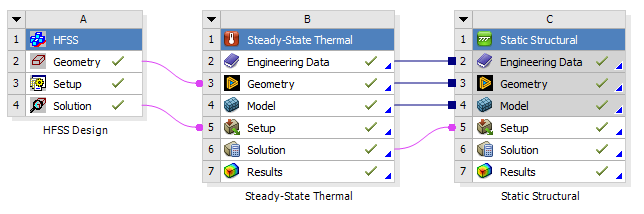
\includegraphics[width=0.5\linewidth]{pic/chapter3/HFSS-ANSYS模块组织.png}
    \caption{ANSYS模块连接方式}
    \label{fig:ANSYSHFSS连接}
\end{figure}

ANSYS中可以直接查看到窗片的应力大小,关于多大的热应力会使得窗片损毁是一个比较经典的材料力学相关问题。当窗片表面的最大最小温度相差过大时,窗片可能会因为温差导致的热应力进而出现损毁,故使用窗片温差来进行窗片损毁判据比较符合直觉。此时根据论文\cite{lishengming_window_2017}中的描述,当窗片的最大最小温度相差达到\(\Delta T\)时,会因为温差导致的热应力而损毁,此时极限温差可以被表述为如下等式\ref{eq:临界温差}所示的形式。其中,\(E\)为材料的弹性模量,\(\sigma_f\)为材料的抗弯强度,\(\alpha\)为热膨胀系数,\(\nu\)为材料的泊松比。
\begin{equation}
    \Delta T = \frac{1 - \nu}{E \cdot \alpha} \sigma_f
    \label{eq:临界温差}
\end{equation}

本次电磁热力联合仿真的频点为9GHz,为工作频段的中心频点附近。此时的仿真馈入功率为14kW,为二次电子发射所计算的最大功率容量。此时关于材料的热与膨胀系数的设置可以参考文章\cite{thumm_stateart_2020},此时设置蓝宝石的密度为\( \rho_{Sapphire}= 4 \times 10^3 kg/ m^3\),各向同性热膨胀系数为\(\alpha{Sapphire} = 5.5 \times 10 ^{-6}K^{-1}\),此时杨氏模量为\( E_{Sapphire}= 385 GPa \),泊松系数为\( \nu_{Sapphire}= 0.22 \),各向同性导热率为\(k_{Sapphire} =900 W/(m \cdot K)\)。此时蓝宝石材料的抗弯强度可以通过文章\cite{hanyong_diff_2011}中找出,此时抗弯系数为\(\sigma_{f} = 320MPa\)。将这些系数输入之后便可以进行稳态热与稳态机械结构的仿真,并且使用公式\ref{eq:临界温差}可以得出此时蓝宝石的温差的极限值为\(\Delta T_{Sapphire} = 117 ^\circ C\),与文章中\cite{hanyong_diff_2011}的计算结果一致。

此时假设窗片外侧的铜制外壳在与空气进行强制对流散热,此时设置铜制外壳的空气对流的热交换系数为\(300 W/ (m \cdot K)\),但是窗片表面由于焊接在器件内部,此时假设其纵向无热对流,并且假设外壳对流的室温为20℃。在设置好期间内部的热交换系数之后,设置波导纵向的两侧端口为固定端面,方便进一步的应力分析。

首先对窗片进行温度场分析,根据图\ref{fig:X输入温度场}显示,此时窗片的温度主要集中于窗片的中心部分,与窗片所传输的电场场强分布相符。并且此时窗片上最大与最小温度差为2℃,小于之前所计算出来的温差的极限值,故窗片已经通过了温度差检验,不会因为温差而导致的热应力所损坏。
\begin{figure}[!htb]
    \centering
    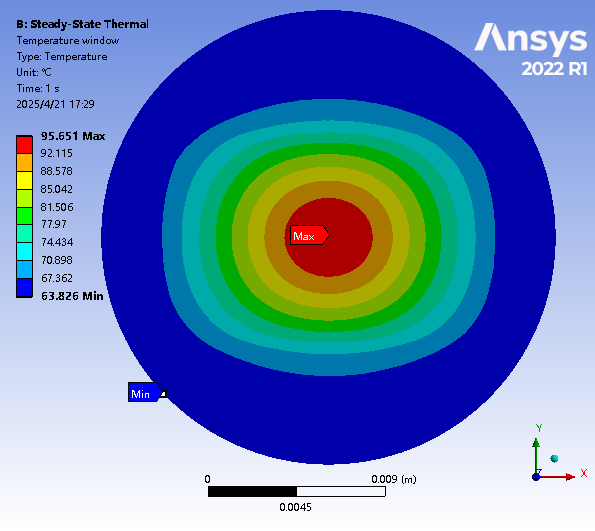
\includegraphics[width=0.5\linewidth]{pic/chapter3/X频段温度分布.png}
    \caption{X输入窗温度分布}
    \label{fig:X输入温度场}
\end{figure}

由于蓝宝石在受热膨胀之后会与外侧的铜制外壳发生挤压,如果挤压的应力过大便会造成窗片损毁,此时使用后续稳态机械求解器所计算的与外侧铜壳之间发生的挤压进而带来的机械应力如图\ref{fig:X输入应力分布}所示。此时最大应力出现在圆形窗与圆角矩形过渡段的接缝处,此时最大应力大小为237MPa。
\begin{figure}[!htb]
    \centering
    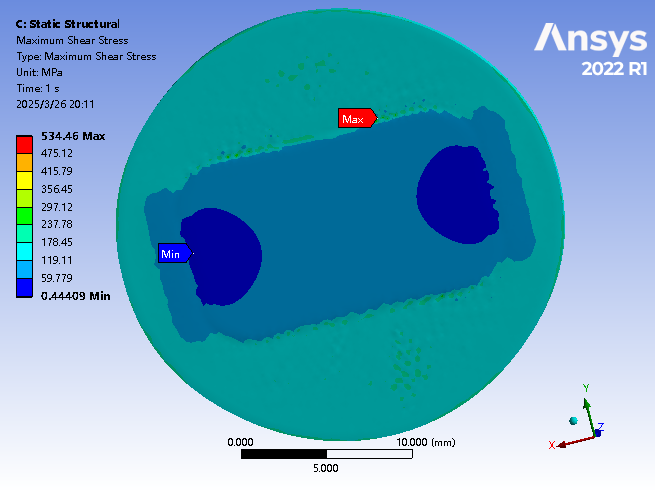
\includegraphics[width=0.5\linewidth]{pic/chapter3/X频段应力分布.png}
    \caption{X输入窗应力分布}
    \label{fig:X输入应力分布}
\end{figure}

关于窗的形变部分,窗片的形变量详见于\ref{fig:X输入窗与波导形变} (a)图中,发现窗片最大形变量为0.0059mm。而窗片与波导整体的形变量详见于\ref{fig:X输入窗与波导形变} (b)图中,窗片与波导整体的最大型变量为0.013mm,波导接触到窗片那一部分的脊处的最大型变量为0.0059mm。结合之前的参数敏感度分析,此形变量较为微小,无法对结构造成能够改变S传输特性的明显变化。综上所述,通过对此时X频段输入窗的多物理场仿真,可以得知此时的窗片设计符合要求。
\begin{figure}[!htb]
    \small
    \centering
    \begin{tabular}{@{\ }c@{\ }c}
        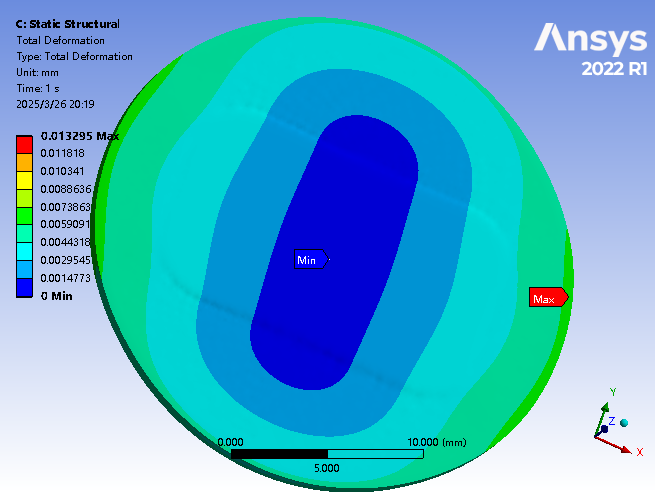
\includegraphics[width=0.4\textwidth]{pic/chapter3/X输入窗总形变.png} & 
        \hspace{5pt}
        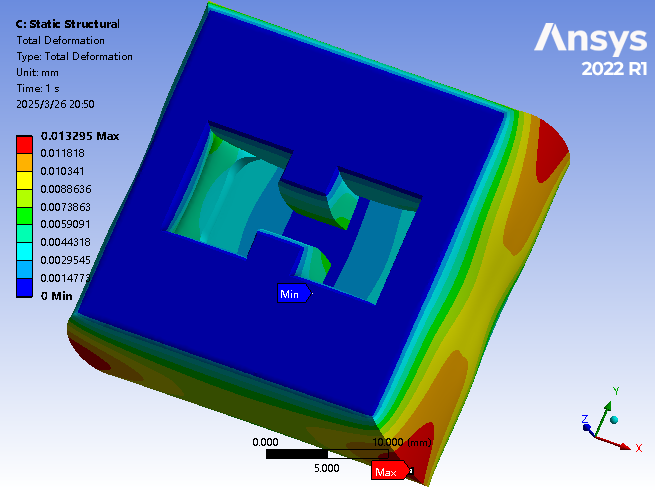
\includegraphics[width=0.4\textwidth]{pic/chapter3/X输入窗与波导.png}     \\
        \mbox{\small (a)X频段输入窗形变}                                                                               & 
        \mbox{\small (b)X频段输入窗与波导形变}                                                                                  \\
    \end{tabular}
    \caption{X频段输入窗与波导形变}
    \label{fig:X输入窗与波导形变}
\end{figure}
        
\section{模式变换部分的设计}
根据之前\ref{fig:6-11GHzDRW}的脊波导几何参数可以看出,此时的脊波导并非公用的标准脊波导,没有标准的同轴转脊波导的模式转换器。如果想要进行进一步的脊波导窗的测试,有必要设计脊波导转同轴的模式转换器。此时结合实际的测试情况,由于之前已经有标准矩形波导转同轴的模式转换器,并且在需要带宽内满足反射系数$S_{11}<-25dB$的反射系数要求。故设计脊波导到标准矩形波导的模式转换器。根据查表显示,标准矩形波导WR112的参数为28.499*12.624mm,本波导的截止频率为5.25GHz,低于所需要频段的最低频点。并且为了标准矩形波导到脊波导之间测试件的纵向长度足够短足够紧凑,本文选取的模式变换主要结构为阶梯过渡,而不是渐变过渡。

[ERRORFIX可能需要补充一点理论相关的。]
经过上述分析,再加上CST方面的优化,得到了如图\ref{fig:脊波导模式变换}所示的模式变换结构:
\begin{figure}[!htb]
    \centering
    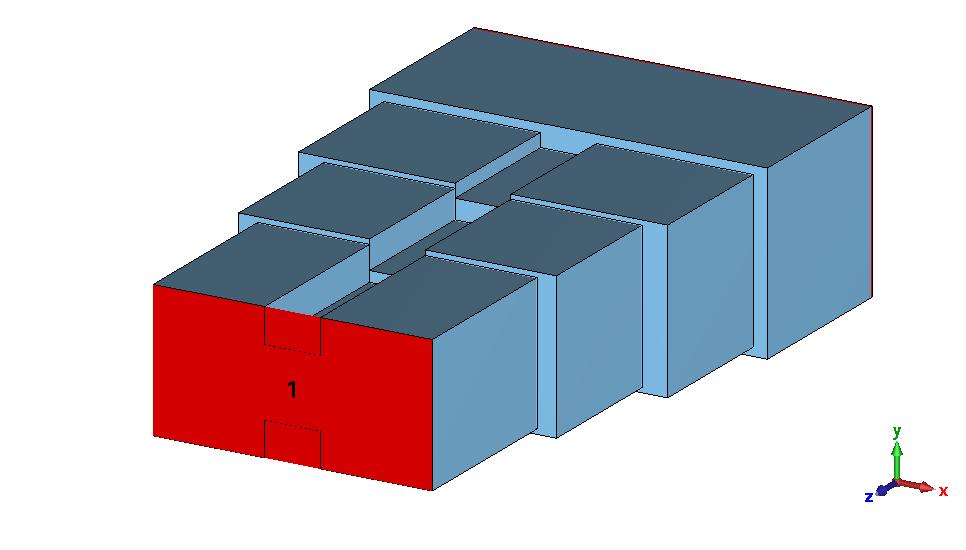
\includegraphics[width=0.5\linewidth]{pic/chapter3/脊波导模式变换.png}
    \caption{脊波导模式变换}
    \label{fig:脊波导模式变换}
\end{figure}
靠近z轴正轴的脊波导为之前\ref{fig:6-11GHzDRW}中所示的双脊波导,而原理z轴正轴的矩形波导纪委之前所提到的WR112标准矩形波导。关于阶梯过度过渡段的各个段落的纵向长度如图片\ref{fig:脊波导模式变换纵向长度} 所示,图中所示的两端过渡段长度均相等,过渡段的总体长度为21.22mm:

\begin{figure}[!htb]
    \centering
    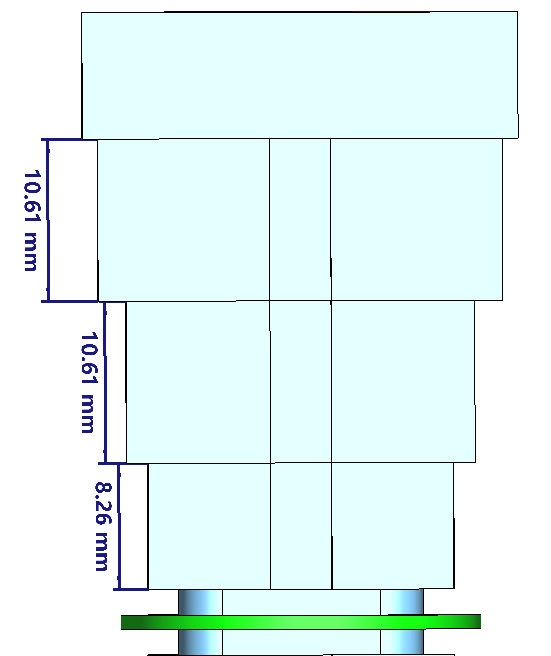
\includegraphics[width=0.5\linewidth]{pic/chapter3/模式变换纵向长度.png}
    \caption{脊波导模式变换纵向长度}
    \label{fig:脊波导模式变换纵向长度}
\end{figure}
此时过渡段中间两个脊波导的脊的宽度与之前所设计的脊波导的脊宽相同,但是脊的高度不同,进而形成阶梯状过渡。过渡段脊波导的空隙高度如图\ref{fig:脊波导模式变换脊的高度}所示:
\begin{figure}[!htb]
    \centering
    
\includegraphics[width=0.25\linewidth]{pic/ERROR.jpg}
    \caption{脊波导模式变换脊的高度}
    \label{fig:脊波导模式变换脊的高度}
\end{figure}

此时过渡段的几何参数已经确定,在将过渡段整体耦合到窗片之前应该单独对过渡段进行S参数仿真。由于1端口(此时为脊波导端口)与2端口(此时为标准矩形波导端口)并不完全一致,故需要分别分析过渡段结构在1端口馈入和2端口馈入时候的情况。仿真结果如图\ref{fig:过渡段不同端馈入的S参数}中所示,其中\ref{fig:过渡段不同端馈入的S参数} (a)展示了脊波导馈入能量时候的S参数,\ref{fig:过渡段不同端馈入的S参数} (b)展示了标准矩形波导馈入能量时候的S参数,此时在两种情况下反射系数$S_{11}$均在频段6-11GHz之内小于-20dB:

\begin{figure}[!htb]
    \small
    \centering
    \begin{tabular}{@{\ }c@{\ }c}
        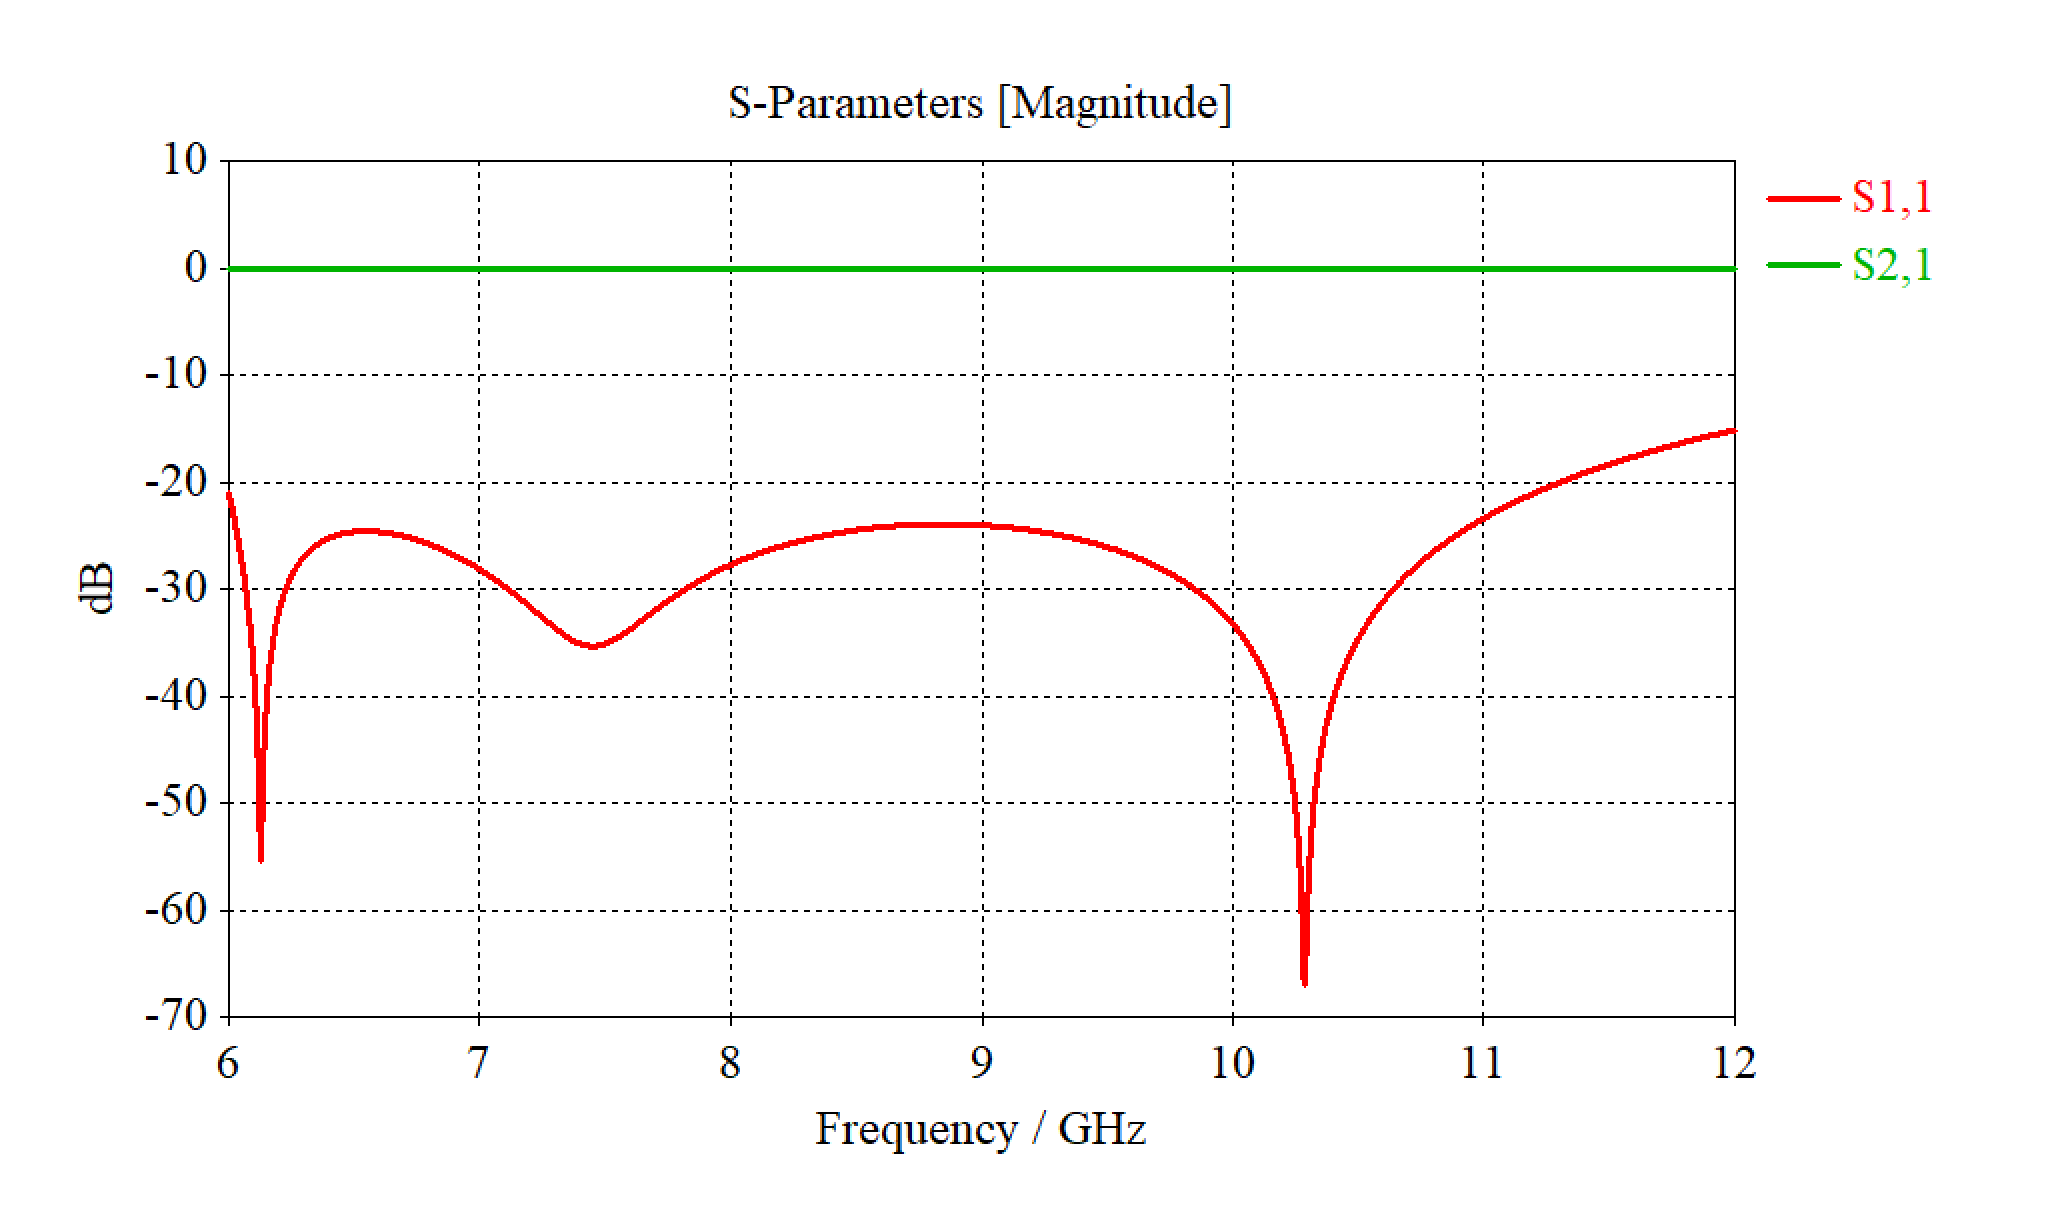
\includegraphics[width=0.49\textwidth]{pic/chapter3/一端口馈入.png} & 
        \hspace{5pt}
        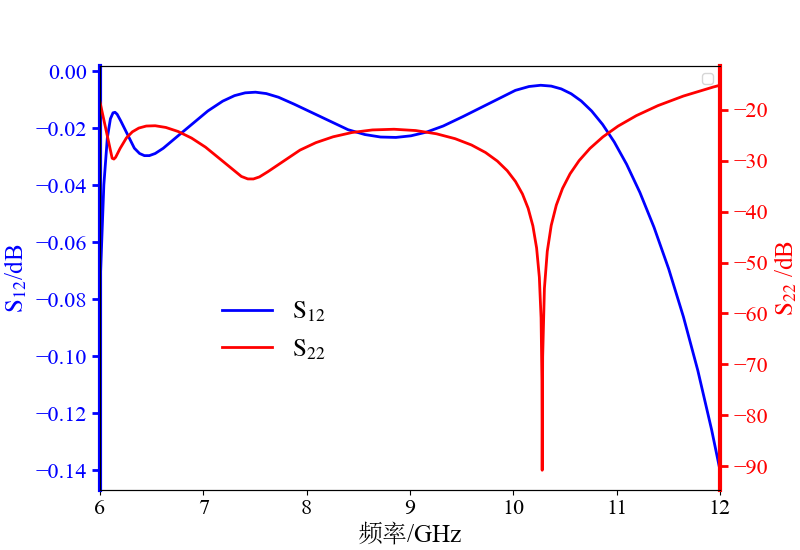
\includegraphics[width=0.49\textwidth]{pic/chapter3/二端口馈入.png}     \\
        \mbox{\small (a)脊波导馈入能量}                                                                               & 
        \mbox{\small (b)标准矩形波导馈入能量}                                                                                  \\
    \end{tabular}
    \caption{过渡段不同端S参数}
    \label{fig:过渡段不同端馈入的S参数}
\end{figure}

此时将过渡段连接到脊波导窗两端,整体的结构如图\ref{fig:脊波导窗的整体测试结构}所示,此时窗片两端均使用阶梯过渡过渡到标准矩形波导WR112。
\begin{figure}[!htb]
    \centering
    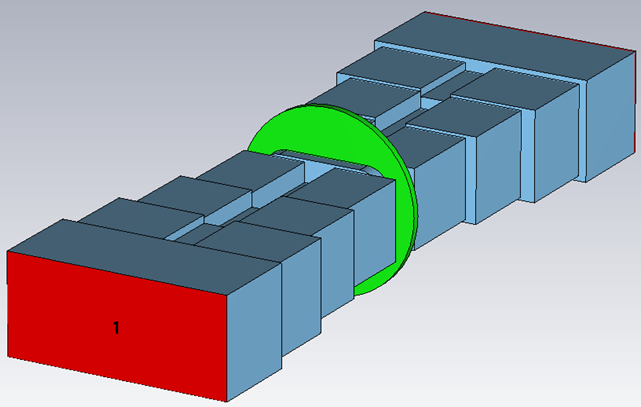
\includegraphics[width=0.5\linewidth]{pic/chapter3/脊波导窗整体测试结构.png}
    \caption{脊波导窗的整体测试结构}
    \label{fig:脊波导窗的整体测试结构}
\end{figure}

此时针对整体接上过渡段之后的窗片进行S参数仿真,得到的结果如图\ref{fig:脊波导窗整体测试结构S参数}所示,此时在频带范围之内(6-11GHz),整体的反射系数也均小于-20dB,满足测试的需求:
\begin{figure}[!htb]
    \centering
    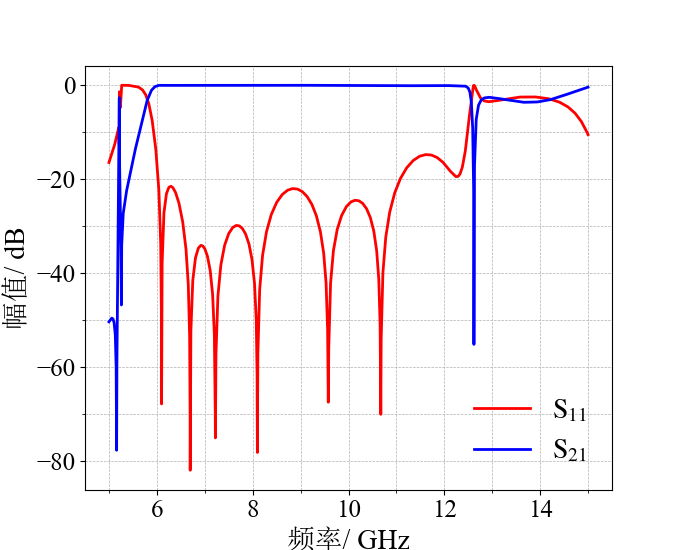
\includegraphics[width=0.5\linewidth]{pic/chapter3/脊波导窗整体S参数.png}
    \caption{脊波导窗整体测试结构S参数}
    \label{fig:脊波导窗整体测试结构S参数}
\end{figure}

\section{小结}
\chapter{L 波段宽频带脊波导窗的设计}
此时仿照之前的6-11GHz 脊波导输入窗进行L 波段宽频带脊波导窗的设计,此时由于需要与前面的L 波段脊波导器件进行直接连接,故L 波段脊波导参数已经被确定,无需对L 波段脊波导进行相应的几何参数设计。关于L 波段脊波导参数,可以见图\ref{fig:L波段脊波导结构} (a)中;图片\ref{fig:L波段脊波导结构} (b)展示了脊波导标红的四条边,这四条边便是脊波导倒圆角的四条边:

\begin{figure}[!htb]
    \small
    \centering
    \begin{tabular}{@{\ }c@{\ }c}
        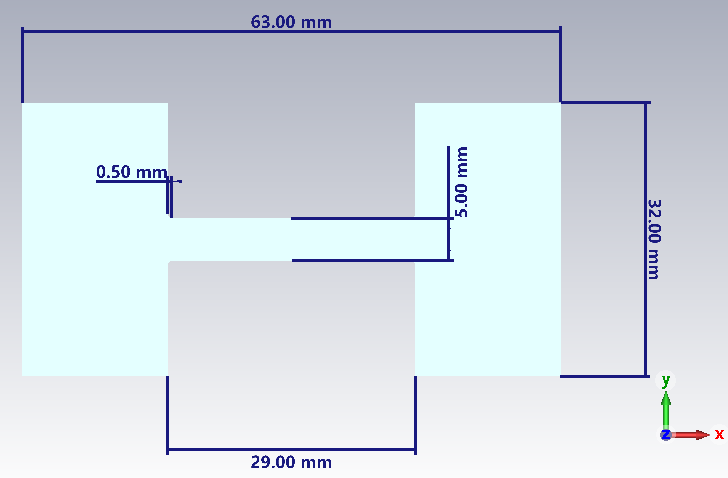
\includegraphics[width=0.45\textwidth]{pic/chapter4/L波段脊波导几何参数.png} & 
        \hspace{5pt}
        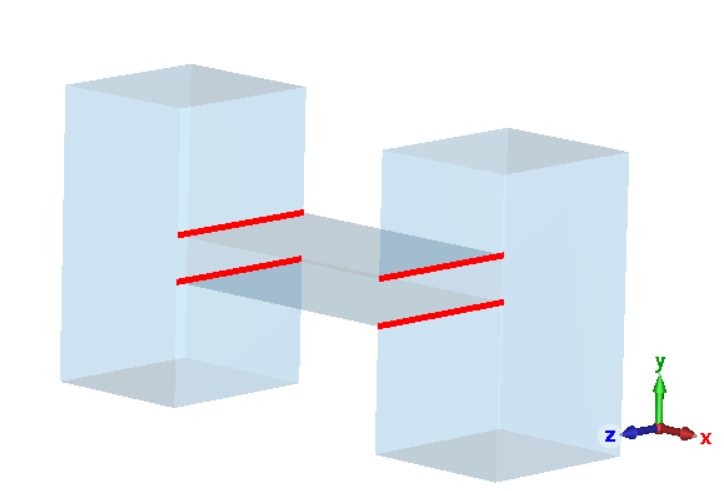
\includegraphics[width=0.45\textwidth]{pic/chapter4/脊波导倒圆角边.png}     \\
        \mbox{\small (a)L波段脊波导几何参数}                                                                               & 
        \mbox{\small (b)脊波导倒圆角的边}                                                                                  \\
    \end{tabular}
    \caption{L波段脊波导结构}
    \label{fig:L波段脊波导结构}
\end{figure}

其中L 波段的脊波导的具体的参数为$a=63mm, b=32mm, s=29mm, d=5mm$此时脊波导为了减少减小最大场强,增大功率容量,防止击穿的考量,在脊波导的两个脊部位进行了倒圆角的设计,倒圆角的尺寸为0.5mm。此时L 波段所需的设计频段为1.14-1.6GHz,此时将脊波导几何参数带入判别式\ref{eq:DRW_constraints}的中进行检验,可以发现此时的$s / a =0.46>0.45$不满足约束条件。但是将\ref{eq:DRW_closed}的算式带入,对L 波段脊波导的截止频率进行计算,可以得到$f_c=1.073GHz$与CST中仿真的结果$1.072GHz$相接近。此时计算脊波导在需要频带内的反射系数可以得到如图\ref{fig:L波段脊波导S参数}的结果:
\begin{figure}[!htb]
    \centering
    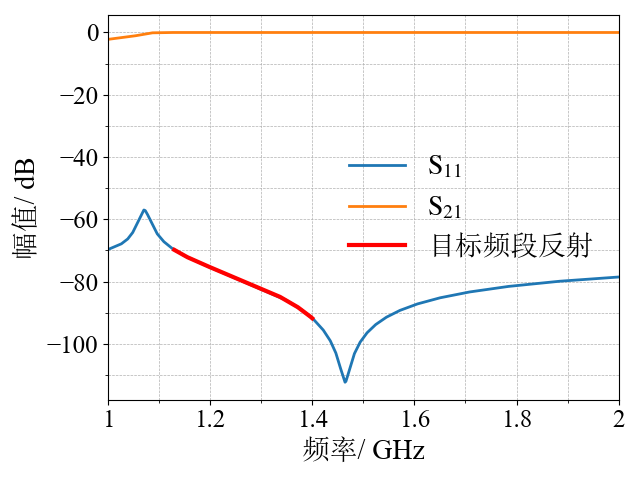
\includegraphics[width=0.5\linewidth]{pic/chapter4/L波段脊波导S参数.png}
    \caption{L波段脊波导S参数}
    \label{fig:L波段脊波导S参数}
\end{figure}。

此时可以看到,在1.13-1.4GHz 的所需频段之内,此时的反射系数$S_{11}<-25dB$,满足匹配要求,可以作为设计窗片所需的脊波导。
\section{频带搬移时候出现的问题分析}\label{sec:频带搬移时候出现的问题分析}
此时仿照之前的6-11GHz 频段所设计的脊波导配圆形窗,并且使用圆角矩形结构作为脊波导和圆窗之间的过渡段进行设计。初步进行频段搬移并且进行优化之后,得到的窗片结构如图\ref{fig:L波段脊波导圆窗的整体结构}所示:
\begin{figure}[!htb]
    \centering
    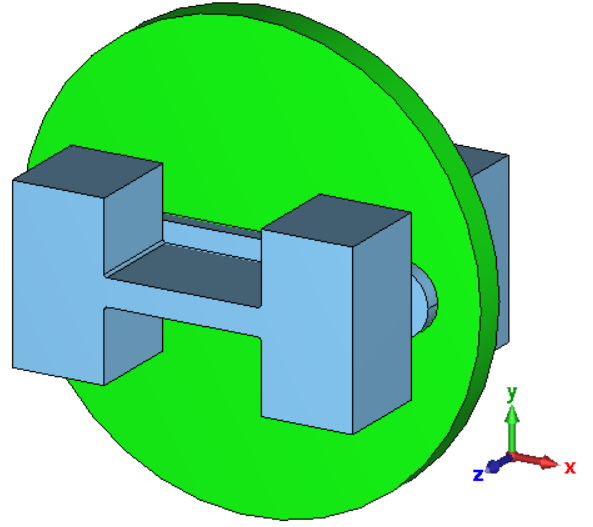
\includegraphics[width=0.35\linewidth]{pic/chapter4/L波段脊波导圆窗的整体结构.png}
    \caption{L波段脊波导圆窗的整体结构}
    \label{fig:L波段脊波导圆窗的整体结构}
\end{figure}

此时窗片的具体几何参数如图\ref{fig:L波段脊波导圆窗的详细几何参数}所示,此时的L波段脊波导窗纵向参数如图\ref{fig:L波段脊波导圆窗的详细几何参数} (a)所示,此时窗片厚度为5.91mm,圆角矩形过渡段的厚度为3.10mm;圆形窗片的直径如图\ref{fig:L波段脊波导圆窗的详细几何参数} (b),圆形窗片的直径为85.14mm;圆角矩形的参数如图\ref{fig:L波段脊波导圆窗的详细几何参数} (c)所示,此时圆角矩形的长边长度为69.2mm,宽边长度为12.63mm,倒圆角的半径为6.41mm。

\begin{figure}[!htb]
    \small
    \centering
    \begin{tabular}{@{\ }c@{\ }c}
        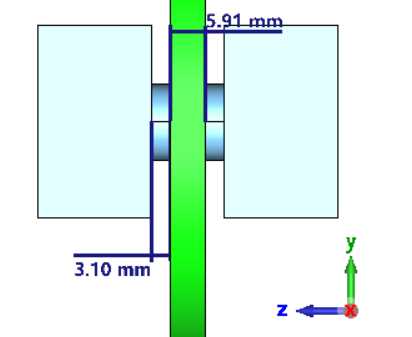
\includegraphics[width=0.19\textwidth]{pic/chapter4/L波段窗纵向长度ORI.png} & 
        \hspace{5pt}
        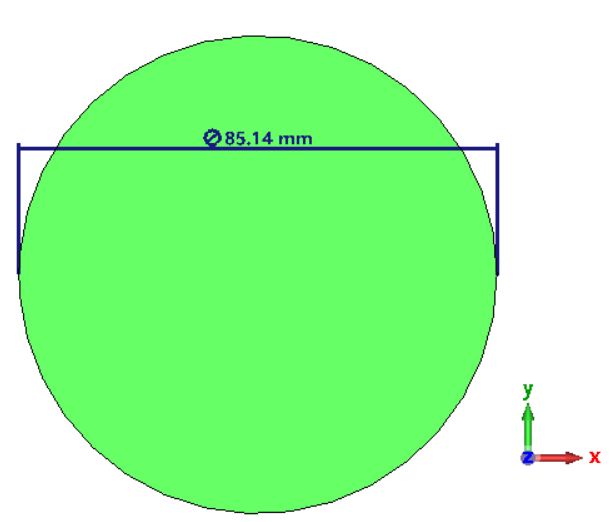
\includegraphics[width=0.19\textwidth]{pic/chapter4/L波段圆形窗片.png}     \\
        \mbox{\small (a)L波段脊波导圆窗纵向长度}                                                                               & 
        \mbox{\small (b)L波段脊波导圆窗参数}                                                           \\[6bp]
        \multicolumn{2}{c}{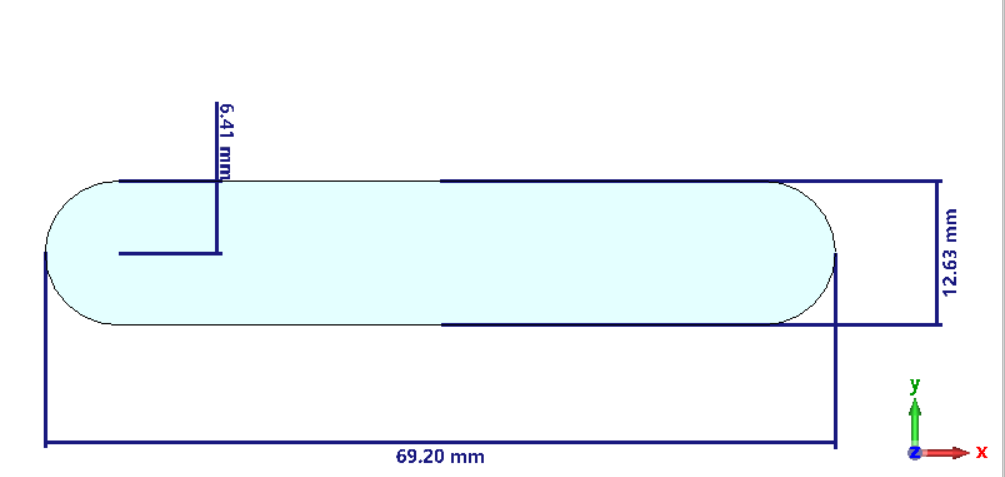
\includegraphics[width=0.35\textwidth]{pic/chapter4/L波段圆角矩形过渡段ORI.png}} \\  % 使用跨列居中
        \multicolumn{2}{c}{\mbox{\small (c)L波段脊波导圆角矩形过渡段参数}}             
    \end{tabular}
    \caption{L波段脊波导圆窗的详细几何参数}
    \label{fig:L波段脊波导圆窗的详细几何参数}
\end{figure}

此时对L 波段脊波导圆窗进行关于S参数的仿真,可以得到S参数如图\ref{fig:L波段脊圆波导窗的S参数}所示,可以看到在1.13-1.4GHz 的频段之内,此时的反射系数$S_{11}<-25dB$,满足匹配要求,可以作为设计窗片所需的脊波导。
\begin{figure}[!htb]
    \centering
    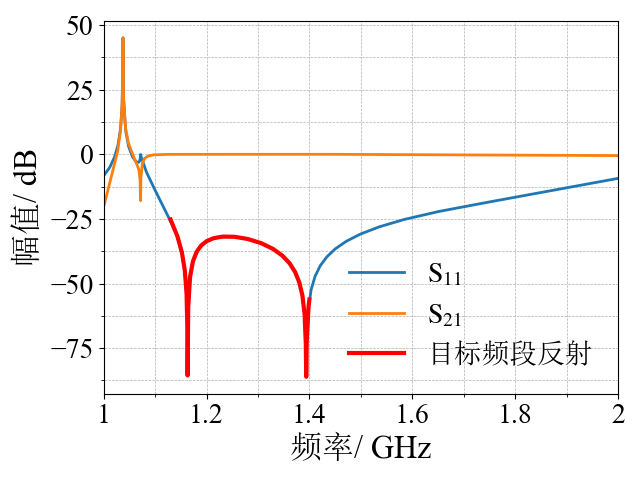
\includegraphics[width=0.45\linewidth]{pic/chapter4/L波段脊圆波导窗的S参数.png}
    \caption{L波段脊圆波导窗的S参数}
    \label{fig:L波段脊圆波导窗的S参数}
\end{figure}

此时设计的脊波导窗虽说在所需要的频段内能够满足$S_{11}$的匹配要求,但是此时的圆形窗片的直径到达了85mm,厚度为5.91mm,此时的圆形窗片实在是过于巨大难以进行加工。并且大窗片更加容易在焊接过程中或者是日常抵挡真空器件的内外压差由于应力过大而发生损坏。针对以上的分析,有必要针对现有的脊波导圆窗结构在L频段施行具体设计时进行相应的改进。

由于此时主要的矛盾集中在窗片过大之上,需要对窗片的场分布进行分析。此时将L波段脊波导圆窗在中轴对称面取横截面,观察截掉之后的电场强度分布如图\ref{fig:L波段脊波导圆窗的电场强度分布}所示。经过观察可以发现,此时窗片在此横截面上面的电场分布更加靠近于脊波导中心处,而圆形窗片的上下两端的电场强度分布并不是特别强。此时可以考虑将圆形窗片的上下两端进行削去,减小窗片在上下的长度,进而减小窗片的体积,使得其结构更加紧凑并且能够加强窗片的机械强度。

并且此时如此之大的蓝宝石窗的加工造价较为昂贵,为了便于进一步的加工设计将窗片的材料更换为氧化铍(BeO) 。此时按照文献[REFERROR]的描述,氧化铍的参数被设置为相对介电常数是$\varepsilon_r = 6.4$ ,损耗角正切是$\tan \delta = 0.0007$ 。

\begin{figure}[!htb]
    \centering
    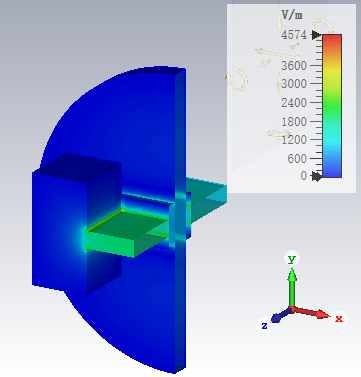
\includegraphics[width=0.35\linewidth]{pic/chapter4/L波段脊波导圆窗的电场强度分布.png}
    \caption{L波段脊波导圆窗的电场强度分布}
    \label{fig:L波段脊波导圆窗的电场强度分布}
\end{figure}

\section{L 波段宽频带脊波导窗的结构设计}
根据之前\ref{sec:频带搬移时候出现的问题分析}节中的分析,此时将从X波段进行频段搬移的窗片结构进行改造。将原先的圆形窗片在电场强度较弱的地方直接进行削除的操作,操作的示意图如图\ref{fig:L频段改造}。示意图中展示了窗片的截面,此时将圆形窗片上下两端以直线进行削除,削除的类似于飞机跑道的结果从外形上看起来更像是倒圆角的矩形。为了方便进一步的加工,此时将不按照被消除上下端的圆窗进行进一步设计,而按照\ref{fig:L频段改造}里面最后的倒圆角的矩形窗片示意图进行进一步地设计。
\begin{figure}[!htb]
    \centering
    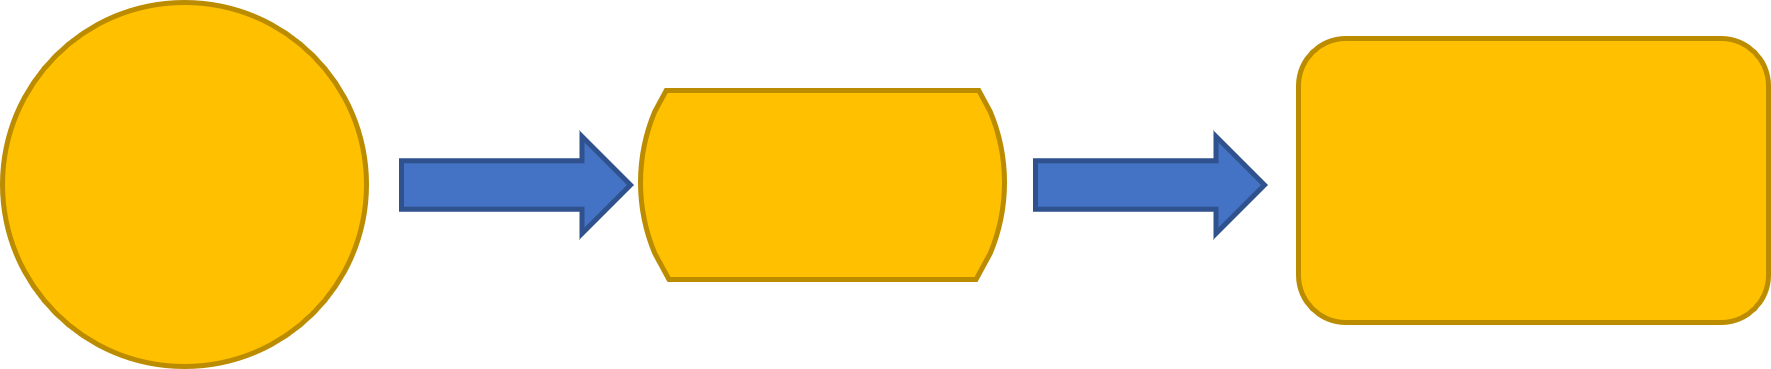
\includegraphics[width=0.5\linewidth]{pic/chapter4/L脊波导窗片改造.png}
    \caption{L频段窗片改造示意图}
    \label{fig:L频段改造}
\end{figure}

在完成之前的设计方案的设计之后的整体窗片结构如图\ref{fig:L波段脊波导窗的整体结构}所示,此时由于脊波导窗的上下端被削去,使得窗的几何结构发生了变化,故两侧的圆角矩形匹配段也会进行重新设计。

\begin{figure}[!htb]
    \centering
    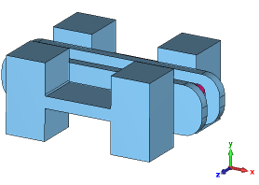
\includegraphics[width=0.3\linewidth]{pic/chapter4/L波段脊波导窗整体结构.png}
    \caption{L波段脊波导窗的整体结构}
    \label{fig:L波段脊波导窗的整体结构}
\end{figure}

此时窗片的详细几何结构参数如图\ref{fig:L波段脊波导窗的详细几何参数}所示,图中\ref{fig:L波段脊波导窗的详细几何参数} (a)展示了窗片的厚度为10.05mm,匹配段的厚度为3.91mm;图中\ref{fig:L波段脊波导窗的详细几何参数} (b)展示了窗片的长度为74.97mm,高度为11.96mm,倒圆角的半径为3.01mm;图中\ref{fig:L波段脊波导窗的详细几何参数} (c)展示了圆角矩形匹配段的长度为87.96mm,高度为20.47mm,倒圆角的半径为7.13mm。
\begin{figure}[!htb]
    \small
    \centering
    \begin{tabular}{@{\ }c@{\ }c}
        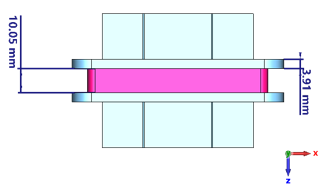
\includegraphics[width=0.19\textwidth]{pic/chapter4/L波段脊波导窗纵向长度.png} & 
        \hspace{5pt}
        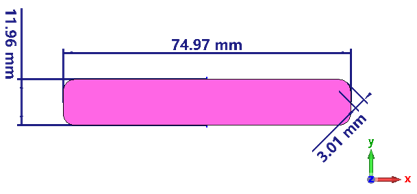
\includegraphics[width=0.19\textwidth]{pic/chapter4/L波段圆角矩形窗片尺寸.png}     \\
        \mbox{\small (a)L波段脊波导窗纵向长度}                                                                               & 
        \mbox{\small (b)L波段脊波导圆角矩形窗参数}                                                           \\[6bp]
        \multicolumn{2}{c}{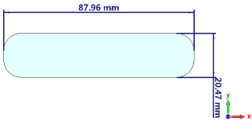
\includegraphics[width=0.35\textwidth]{pic/chapter4/L波段过渡段尺寸.png}} \\  % 使用跨列居中
        \multicolumn{2}{c}{\mbox{\small (c)新设计L波段脊波导圆角矩形过渡段参数}}             
    \end{tabular}
    \caption{L波段脊波导窗的详细几何参数}
    \label{fig:L波段脊波导窗的详细几何参数}
\end{figure}


为了验证新设计的脊波导窗的实际性能,我们对其S参数进行了仿真分析,并得到了如图\ref{fig:L波段脊波导窗的S参数}所示的结果。仿真结果显示,在目标频段内,该设计的反射系数$S_{11}$成功降至-20dB以下,满足了严格的匹配要求。除了保持原有的性能指标外,新款窗口还展示了更小巧的尺寸和更加紧密的结构布局,这无疑为实际应用提供了更多的灵活性。更重要的是,此次设计上的革新简化了制造流程,提升了机械强度,从而保证了产品在各种环境下的稳定表现。

\begin{figure}[!htb]
    \centering
    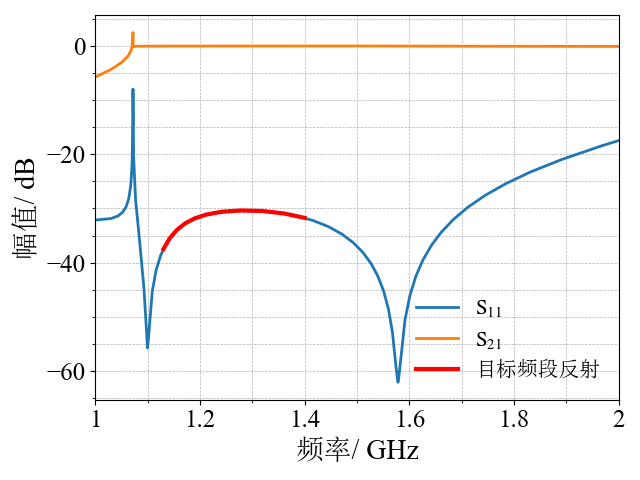
\includegraphics[width=0.45\linewidth]{pic/chapter4/L波段脊波导窗S参数.png}
    \caption{L波段脊波导窗的S参数}
    \label{fig:L波段脊波导窗的S参数}
\end{figure}
\section{计算L波段脊波导窗功率容量}
\subsection{使用最大场强法计算脊波导窗的功率容量}
\subsection{使用电子倍增计算脊波导窗的功率容量}

使用电子倍增方法来计算L波段脊波导窗的方法与X波段的大致相同,首先选取的二次电子发射模型依然是Vaughan模型。此时选用的铜的二次电子发射曲线依然跟原先X波段的相同,但是此时选择氧化铍(BeO)相关的二次电子发射曲线必须重新检索文献并且使用文献中的结果。此时根据文献\cite{shih_1994_beosee}中的数据,BeO的二次电子发射曲线的关键参数为$\delta_{max}=2.8 \pm 0.1, E_{max}=420 \pm 20 eV, E_1 = 40 \pm 2 eV$,本文献实验的入射电子的能量范围为从10到2900eV;根据文献\cite{ritz_1988_secondary}中的记述,关键参数为$\delta_{max}=2.27, E_{max}= 443  eV, E_1 =54.9 eV$,测试的入射电子能量范围为从10到900eV。综合上述文献的参数,此时将BeO的二次电子发射曲线在Vaughan模型中的关键参数设定为$\delta_{max}=2.8 , E_{max}=420 , E_1 = 40 eV$,并且入射电子的能量范围为从10到2900eV,设置好关键参数之后的曲线如图\ref{fig:BeO二次电子发射曲线}所示。
\begin{figure}[!htb]
    \centering
    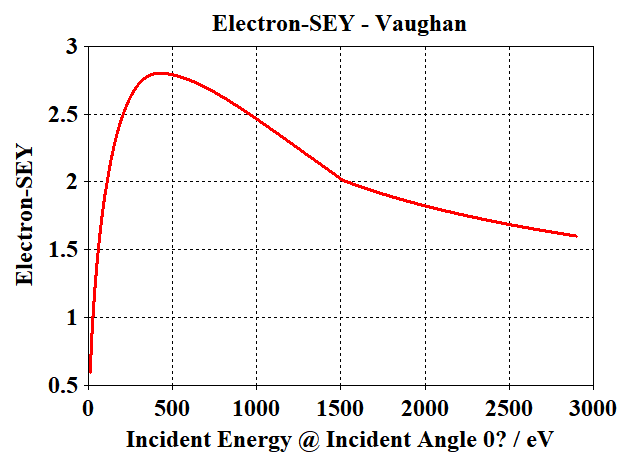
\includegraphics[width=0.5\linewidth]{pic/chapter4/BeO二次电子发射曲线.png}
    \caption{BeO二次电子发射曲线}
    \label{fig:BeO二次电子发射曲线}
\end{figure}

此时为了方便设置Spark3D和CST中的PIC模块中的材料的二次电子发射曲线,在床片外侧套了一层矩形的铜制外壳,矩形外层的最窄数值为2mm。在加入铜制外壳之后,窗片的整体结构如图\ref{fig:L波段加上铜制外壳}所示。

\begin{figure}[!htb]
    \centering
    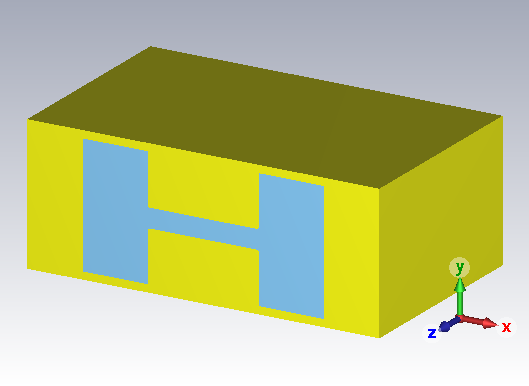
\includegraphics[width=0.3\linewidth]{pic/chapter4/L波段加上铜制外壳.png}
    \caption{L波段脊波导窗加上铜制外壳的整体结构}
    \label{fig:L波段加上铜制外壳}
\end{figure}

在套上铜制外壳之后,由于窗片在低频点更容易被击穿,故在所需频段的最低频点1.14GHz频点导出Spark3D所需的电场与磁场结果。并且为了查看铜制外壳是否会对窗片的S曲线产生影响,对加上铜制外壳后的窗片的S曲线进行了仿真,仿真的结果如图\ref{fig:L波段加上铜外壳后的S参数}所示。仿真结果显示,铜制外壳对窗片的S参数并没有明显的影响。

\begin{figure}[!htb]
    \centering
    \includegraphics[width=0.45\linewidth]{pic/chapter4/L波段加上铜外壳后的S参数.png}
    \caption{L波段加上铜外壳后的S参数}
    \label{fig:L波段加上铜外壳后的S参数}
\end{figure}

此时对导入Spark3D之后的电场强度进行观察,观察结果图\ref{fig:L波段Spark3D仿真结果} (a)所示,此时窗片整体中电场强度较高的部分集中在脊波导窗片的脊之间,其次便是脊波导与窗片之间过渡段靠近脊波导的那一条边,这个仿真结果与X波段中脊波导窗的仿真结果相类似。此时在Spark3D中按照之前所查到的参数,设置好每一种材料的二次电子发射系数。并且将馈入窗的能量设置为1.14GHz连续波,此时由于Spark3D中的电子为随机散布,为了确保仿真结果的准确性相比于Spark3D的初始电子数目三百进行相应的增加,于是将窗中的初始电子数目设置为8000。在Spark3D中进行好上述材料的曲线设置之后,此时判断击穿的标准依然是窗的电子数目随着时间的变化呈现出下降的趋势及被视为不被击穿,如果呈现出如指数一般的急剧上升趋势或者先下降后上升的趋势则被视为已经击穿。观察此时如图\ref{fig:L波段Spark3D仿真结果} (b)的Spark3D的仿真结果,可以看到此时的窗的功率容量为1012W。

\begin{figure}[!htb]
    \small
    \centering
    \begin{tabular}{@{\ }c@{\ }c}
        \includegraphics[width=0.49\textwidth]{pic/chapter4/L波段Spark3D电场.png} & 
        \hspace{5pt}
        \includegraphics[width=0.49\textwidth]{pic/chapter4/Spark3D中的电子随时间的变化.png}     \\
        \mbox{\small (a)Spark3D中的电场强度}                                                                               & 
        \mbox{\small (b)Spark3D中的电子随时间的变化}                                                                                  \\
    \end{tabular}
    \caption{L波段Spark3D仿真结果}
    \label{fig:L波段Spark3D仿真结果}
\end{figure}

有了之前的Spark3D所展示的基于电子倍增效应计算的功率容量的仿真结果,此时可以进行CST中使用PIC求解器进行关于电子倍增效应。首先根据之前的仿真结果,应该将初始电子填充在窗片的脊波导的脊与脊波导和窗片之间的过渡段之中,具体的填充区域如图\ref{fig:L波段CST电子填充方法}所示,为了保证求解的真实可靠性,综合前面的分析,本次每个区域中填充电子的密度不低于$10^9 m^{-3}$。
\begin{figure}[!htb]
    \centering
    \includegraphics[width=0.25\linewidth]{pic/chapter4/L波段CST电子填充方法.png}
    \caption{L波段CST中PIC的初始电子填充区域}
    \label{fig:L波段CST电子填充方法}
\end{figure}

在完成了PIC求解器中的电子填充之后,此时便可以设置激励信号进行仿真。由于期间比较容易在低频点击穿,故此时设置的连续波的频率为1.14GHz。并且在进行一些初步仿真之后发现初始电子的消失时间大概为150ns,为了确保查看电子数目随着时间的变化的趋势足够充分,故总仿真时长不应低于初始电子消失时间的两倍,本次仿真的总时长被设定为320ns。经过不同功率1.14GHz连续波的激励之后,查看器件中电子数目随着时间的变化趋势如图\ref{fig:L波段PIC基于二次电子仿真计算功率容量结果}所示。综上上述分析,此时的器件的功率容量大致上为1175W。
\begin{figure}[!htb]
    \centering
    \includegraphics[width=0.5\linewidth]{pic/ERROR.jpg}
    \caption{L波段PIC基于二次电子仿真计算功率容量结果}
    \label{fig:L波段PIC基于二次电子仿真计算功率容量结果}
\end{figure}

\section{关于L波段脊波导窗片的多物理场分析}
类似于之前的小节,本小节针对L波段脊波导窗进行了多物理场的分析,此时针对BeO材料的特性主要参考为文献\cite{thumm_stateart_2020, slack_thermal_1971,kozlovskii_thermal_2014,hanyong_diff_2011}中所记述的实验数据。综合上述论文中的实验数据,将BeO的关键参数设置如下密度\(\rho_{BeO} = 2850kg/m^3\),热膨胀系数为\(\alpha = 7.2 \times 10^{-6} K^{-1}\),杨氏模量为\(E_{BeO} = 385GPa\),泊松系数为\(\nu_{BeO} = 0.3\),导热系数为\(k_{BeO} = 260 W/(m \cdot K)\)。此时BeO的抗弯系数为$\sigma_f = 200MPa$,故此时根据公式\ref{eq:临界温差}可以计算其最大最小温度极限差值为45℃,如果窗片的温差超过45℃那么便有因为温差过大进而导致热应力过大,进而引起窗片碎裂的风险。

此时窗片HFSS中馈入频点为中心频点1.3GHz,馈入的功率为1kW,接近于PIC求解器所求的窗片的功率容量上限。此时为了方便窗片的应力仿真,将窗片的外壳两端的端面设置为固定的端面。此时仿真得到的窗片的温度场如图\ref{fig:L频段窗温度分布}所示,此时窗片的温度集中于窗片的中心部分,此时中心部分的场强也更强损耗也更大,满足仿真结果预期。此时窗片上最大温度为20.61℃,最小值为20.53℃,温差为0.08℃,此时温差小于之前所计算的温差极限值,此时窗片通过了温差检验。
\begin{figure}[!htb]
    \centering
    \includegraphics[width=0.5\linewidth]{pic/chapter4/L频段窗温度分布.png}
    \caption{L频段窗温度分布}
    \label{fig:L频段窗温度分布}
\end{figure}

此时导出窗片应力分布,可以得到窗片的应力分布如图\ref{fig:L频段窗应力分布}所示,此时窗片的最大应力为3.76MPa。出现最大应力部分主要为窗片与脊波导之间的过渡段,即窗片与铜制外壳直接接触的面。
\begin{figure}[!htb]
    \centering
    \includegraphics[width=0.5\linewidth]{pic/chapter4/L频段窗应力.png}
    \caption{L频段窗应力分布}
    \label{fig:L频段窗应力分布}
\end{figure}

此时导出窗片与整体的形变分布,可以得到如图\ref{fig:L频段窗与整体形变分布}所示的窗片与整体的形变分布,此时根据图\ref{fig:L频段窗与整体形变分布} (a)中的数据,窗片的形变量最大为\(5 \times 10 ^{-4}mm\)。窗片整体的形变量分布如图\ref{fig:L频段窗与整体形变分布} (b)所示,此时窗片整体的形变量最大为\(1 \times 10 ^{-3}mm\),结合之前的参数敏感度分析,此时窗片的形变量不应该对窗片的性能造成较大的影响。综上所述,此时窗片能够在1.3GHz频点处满足1kW功率的要求。
\begin{figure}[!htb]
    \small
    \centering
    \begin{tabular}{@{\ }c@{\ }c}
        \includegraphics[width=0.49\textwidth]{pic/chapter4/L频段窗形变.png} & 
        \hspace{5pt}
        \includegraphics[width=0.49\textwidth]{pic/chapter4/L频段整体形变.png}     \\
        \mbox{\small (a)L频段窗形变}                                                                               & 
        \mbox{\small (b)L频段窗与波导形变}                                                                                  \\
    \end{tabular}
    \caption{L频段窗与波导整体形变分布}
    \label{fig:L频段窗与整体形变分布}
\end{figure}


\section{小结}
\chapter{窗片测试过程中的误差分析}
\section{6-11GHz脊波导窗片旋转误差分析}\label{sec:6-11GHz脊波导窗片旋转误差分析}
在之前的章节中,已经针对6-11GHz频段的窗片进行了参数敏感度相关的分析,但是还未对其可能的装配误差进行进一步的分析。在实际的窗片焊接过程中,旋转误差是一种常见的装配误差,现在以6-11GHz频段的脊波导窗片为例,以一种比较简单的情况针对装配的旋转误差造成的结果进行引入。首先假设此时此脊波导窗脊波导的长边位于x轴之上,并且电磁波的传输方向为z轴的方向(在CST中进行实际建模时候也确实如此)。圆形窗片首先绕着x轴发生了角度为$\theta=3^ \circ $的旋转,在进行完这一个方向的旋转之后绕着全局坐标中的z轴发生了角度为$\psi$从$0^ \circ$到$180^ \circ$步长为$45^ \circ$的一系列旋转。每次$\psi $步进完成之后都使用CST对窗片的S参数进行仿真,并且将仿真结果对反射系数$S_{11}$进行记录,最后记录的$S_{11}$参数见图\ref{fig:脊波导圆窗旋转}之中。
\begin{figure}[!htb]
    \centering
    \includegraphics[width=0.5\linewidth]{pic/chapter5/脊波导圆窗旋转.png}
    \caption{脊波导窗装配旋转误差分析}
    \label{fig:脊波导圆窗旋转}
\end{figure}

仔细观察仿真完成后的曲线发现,此时$S_{11}$曲线根据$\psi$的变化而产生周期性的变化,大致上可以把发生旋转之后的图片分为三类,即$\psi = 0 ^\circ$或者$180 ^\circ$为一组,$phi = 45 ^\circ$和$135 ^\circ$为一组,最后$phi = 90 ^\circ$和未发生旋转的为一组,分组的结果详见图片\ref{fig:脊波导圆窗旋转分组}。
\begin{figure}[!htb]
    \centering
    \includegraphics[width=0.5\linewidth]{pic/ERROR.jpg}
    \caption{脊波导窗装配旋转误差分析分组}
    \label{fig:脊波导圆窗旋转分组}
\end{figure}

$S_{11}$曲线根据$\psi$出现周期性的变化的原因是脊波导传输的模式为类$TE_{01}$模式,这个模式类似于矩形波导的$TE_{01}$模式,是一种线极化模式。这种线极化模式使得窗片的工作性能不仅仅与最开始窗片绕着x轴旋转的角度$\theta$相关,也与窗片后续绕着全局坐标轴z转动的角度$\psi$相关。值得注意的是由于圆形窗片的圆对称性质,并不需要完全引入刚体旋转欧拉角的三根不同的坐标轴进行分析。原因是由于需要考虑线极化模式类$TE_{01}$模式的影响,窗片最后绕着旋转变换一定是绕着全局坐标轴z轴进行角度为$\psi$的旋转,而前面绕着全局坐标轴x和y进行的旋转变换都可以由于圆形窗片的圆对称性质化归为绕着x轴进行角度为$\theta$的旋转变换加上绕着全局坐标轴z轴进行一定角度的旋转。

由此可见,圆形窗片的旋转装配误差并不单单只是跟窗片绕着x轴的倾斜角$\theta$相关,也会跟窗片绕着z轴旋转的角度$\psi$相关。
\section{W频段95GHz窗片测试误差分析}
针对W频段的95GHz圆形窗片进行测试,测试时候的示意图如图\ref{fig:W频段测试示意图}所示。此时窗被焊接在一个方圆渐变段的圆形那一段的顶部,渐变段的另一端是一标准矩形波导WR-8,其尺寸为$2.58mm \times 1.27mm$,标准矩形波导后续部分便接上同轴过渡段进而接到矢量网络分析仪中。渐变段另一端的圆端则是直接通往大气,为了匹配,渐变段的顶端往外延伸了一段匹配圆柱形波导。此时匹配圆柱的直径和窗片的直径都是16mm,匹配圆柱的长度是8.447mm,蓝宝石窗片的厚度是1.035mm,渐变过渡段的长度是126.99mm。
\begin{figure}[!htb]
    \centering
    \includegraphics[width=0.5\linewidth]{pic/chapter5/W频段测试示意图.png}
    \caption{W频段测试示意图}
    \label{fig:W频段测试示意图}
\end{figure}

\subsection{窗片测试与仿真的不一致性}

首先对窗片进行反射系数$S_{11}$的测试时发现,窗片相对于原先在理想情况下仿真得到的在95GHz处的匹配频点,实际测试的窗的谐振频点略微往下漂移1GHz,反射系数匹配的频点位于94GHz处。具体的测试图片如图\ref{fig:W波段实际测试结果}所示。但是此时在95GHz处的反射系数为-25dB,符合反射系数要求,在此频点处可以正常使用。
\begin{figure}[!htb]
    \centering
    \includegraphics[width=0.35\linewidth]{pic/chapter5/实际测试的W波导窗.jpg}
    \caption{W波段实际测试结果}
    \label{fig:W波段实际测试结果}
\end{figure}

并且在实际测试时,如果将信号传输方向定义为z轴方向,发现窗片和过渡段在绕着z轴旋转时候时反射系数会周期性的发生变化。如果将反射系数$S_{11}$数据最好的旋转角度定义为0°的话,当旋转角度达到90°时,$S_{11}$的反射情况会到达最差,最差时候在95GHz频点处的反射系数值系数值只有15dB。并且旋转到45°和135°时候的反射系数值是一致的,在到达67.5°和112.5°时候反射系数也是一致的,简要来说的话测试时候得到的反射系数的值的旋转角度关于90°对称。

具体测试环境下的图片如图\ref{fig:W频段反射与旋转角度关系}所示,为了使得仿真过程中的旋转角度能够更方便的被看到,在旋转到反射系数旋转到达最佳值的时候在窗片某一个的孔位上面放了一颗螺丝钉作为标记。此时测试过程中旋转的角度已经使用文字在图中进行了相应的标注。
\begin{figure}[!htb]
    \centering
    \includegraphics[width=0.55\linewidth]{pic/chapter5/W频段反射系数与旋转角度关系.png}
    \caption{W频段反射系数与旋转角度关系}
    \label{fig:W频段反射系数与旋转角度关系}
\end{figure}

\subsection{针对不一致性的仿真分析}
此时猜测匹配的频偏是由于装配误差和矩形-圆波导过渡段所共同造成的,并且结合之前小节\ref{sec:6-11GHz脊波导窗片旋转误差分析}的分析,可以看到此时的装配误差和绕z轴旋转的角度周期性的相关。此时初步推测是由于圆形窗片在装配过程中引起的装配误差是旋转误差,进而引起了这种周期性的误差。

此时使用高度规针对窗片顶面进行高度测量,此时测量出来窗片顶面圆周相对于圆心在z轴方向上有着一定的高度差,具体的圆周相对于圆心的高度差如图\ref{fig:W频段圆周高度差测试结果}所示。此时关于度数的定义与之前相同,窗片反射系数$S_{11}$测试结果最好的地方定义为0°,并且按照逆时针逐渐增大,每旋转45°测量一次窗片顶面圆周相对于圆心的高度差。经过高度规的测试发现,此时的高度差随着角度的变化而呈现出正弦幅值的变化,合理推测此时窗片发生了旋转,但是具体的旋转方向与装配的旋转角度仍需要进一步的预估计算。
\begin{figure}[!htb]
    \centering
    \includegraphics[width=0.5\linewidth]{pic/chapter5/可视化高度差.png}
    \caption{W频段圆周高度差测试结果}
    \label{fig:W频段圆周高度差测试结果}
\end{figure}

假设此时窗片发生了过圆柱体顶面中心的旋转,旋转轴位于窗片顶面的平面之内,相对于标定的0°的偏离角度是$\psi$,此时窗片绕着旋转轴旋转的角度为$\theta$,窗片的半径为R。此时假设旋转之后的圆面上有一点P,现在假设P点在旋转之前跟x轴之间的夹角为\(\alpha \)。此时窗片发生过圆心的旋转的装配误差情况可以按照示意图\ref{fig:过圆心旋转示意图}所示。
\begin{figure}[!htb]
    \centering
    \includegraphics[width=0.5\linewidth]{pic/chapter5/过圆心旋转示意图.png}
    \caption{窗片过圆心旋转示意图}
    \label{fig:过圆心旋转示意图}
\end{figure}

根据之前的定义,此时旋转轴的方向向量为 \(\mathbf{k} = (\cos\psi, \sin \theta, 0)\),旋转前的OP坐标为\(\mathbf{v} = (R\cos \alpha, R\sin \alpha, 0)\),旋转为OP的向量$\mathbf{v}$绕着旋转轴的方向向量\(\mathbf{k}\)旋转了\(\theta \)角。此时使用罗德里格斯旋转公式,公式可以见于\ref{eq:罗德里格斯旋转公式},来对旋转之后的点的向量进行计算。
\begin{equation}\label{eq:罗德里格斯旋转公式}
    \mathbf{v}_{rot} = \cos\theta \cdot \mathbf{v} + (1 - \cos\theta) \cdot (\mathbf{v} \cdot \mathbf{k}) \mathbf{k} + \sin\theta \cdot (\mathbf{k} \times \mathbf{v})
\end{equation}

根据上述进而可以得知此时P点旋转之后的向量值,直接截取旋转后的向量值\(\mathbf{v}_{rot}\)的z轴的值即为P点偏离原先平面的z值的长度为如公式\ref{eq:deltaz_center}所示。
\begin{equation}\label{eq:deltaz_center}
    \Delta z = R \sin \theta \sin \left(\alpha -\psi \right)
\end{equation}

时根据已经测量得到的数据结合几何知识所计算出来了的公式并且使用Python代码进行拟合,可以得到\( \psi = 208.8 ^ \circ, \theta = -0.00369rad \),此时将拟合得到的值重新带入计算公式\ref{eq:deltaz_center}进行计算并且进行将拟合结果和测量结果进行对比并且作图,得到如图\ref{fig:过圆心高度差拟合结果}所示的结果,从图中可以看到拟合的效果并不理想。于是怀疑此时窗片的旋转轴偏离了圆心,而不是之前所猜测的过圆心的旋转。
\begin{figure}[!htb]
    \centering
    \includegraphics[width=0.5\linewidth]{pic/chapter5/过圆心高度差拟合.png}
    \caption{过圆心高度差拟合结果}
    \label{fig:过圆心高度差拟合结果}
\end{figure}

此时设定测量的反射系数结果最好的那个方向为x轴,窗片顶面所在平面为xOy平面,窗片顶面与底面的法向量为z轴所在的法向量。此时假设圆窗片的上面沿着直线l发生弧度为\(\theta\)的旋转,此时直线l到圆心的最短距离是d,直线l与x轴的夹角为\(\psi\)。此时偏离圆心的旋转的情况可以见于示意图\ref{fig:旋转轴偏离圆心的旋转情况}。
\begin{figure}[!htb]
    \centering
    \includegraphics[width=0.5\linewidth]{pic/chapter5/不过圆心旋转示意图.png}
    \caption{旋转轴偏离圆心的旋转情况}
    \label{fig:旋转轴偏离圆心的旋转情况}
\end{figure}

值为那么此时直线在xOy平面上的方程可以被表示为\(x \sin \psi - y \cos \psi = d\),直线的方向向量为 \(\mathbf{k} = (\cos \psi, \sin \psi, 0)\),通过点 \(P_0 = (d \sin\psi, -d\cos\psi , 0)\),此点为原点到直线所引垂线垂足的坐标。此时我们要计算绕着方向向量旋转的点的坐标,需要使用罗德里格斯旋转公式,但是在那之前需要先使用坐标变换将圆上面的点的坐标平移到以\(P_0\)为原点的坐标系。假设圆面上点在发生旋转之前的坐标是\(P = (x,y,0)\),变换之后的向量变为\(\mathbf{v} = (x - d\cos\psi, y + d\sin\psi, 0)\)。此时再应用旋转公式\ref{eq:罗德里格斯旋转公式},将向量\(\mathbf{v}\)转化为旋转后的向量\(\mathbf{v}_{rot}\)。此时只需要截取向量\(\mathbf{v}_{rot}\)的z轴的值即可计算出来P点偏移之后的偏移量\(\Delta z\),此时求出结果后的值如式子\ref{eq:不过圆心直角坐标系中的z值}所示:
\begin{equation}\label{eq:不过圆心直角坐标系中的z值}
    z' = \sin \theta \left(d + \cos\psi \cdot y - \sin\psi \cdot x \right)
\end{equation}
但是由于圆上面的点P的坐标满足\(x = R\cos\alpha\),\(y = R\sin\alpha\),其中\(\alpha\)是旋转之前的点的极角,将其带入式子\ref{eq:直角坐标系中的z值}中,得到旋转之后的点的z坐标的值与原先点的极角\(\alpha\)之间的关系,计算完成后的结果如式子\ref{eq:不过圆心旋转之后的z值}所示:
\begin{equation}\label{eq:不过圆心旋转之后的z值}
    \Delta z = z' = \sin \theta \left[d+R \sin (\alpha -\psi )\right]
\end{equation}

式子中,\(\theta\)是窗片旋转的角度,\(\psi\)是旋转轴与x轴的夹角,\(d\)是圆心到旋转轴的距离,\(\alpha\)是旋转前圆窗片上的点P的极角。此时为了检验计算的结果,将式子\ref{eq:不过圆心旋转之后的z值}中的d值赋值为0,将结果与式子\ref{eq:deltaz_center}中的结果作为对比,发现一致的,证明计算结果自洽。

此时需要用原先测试的偏移值来估计\(\theta, \psi\)以及\(d\)的值,此时需要使用线性拟合的方法来进行计算。仔细观察式子\ref{eq:不过圆心旋转之后的z值}可以发现\(\Delta z\)可以被转化为线性形式,此时\(\Delta z =A+B \cos \alpha +C \sin \alpha \),其中\(A = \sin \theta \cdot d, B = -R \sin \theta \sin \psi, C = -R \cos \psi \sin \theta \)。此时根据给定的测量的高度差数据可以对给定的系数\(A, B, C\)使用最小二乘法进行拟合,最后使用系数\(A, B, C\)来进行参数化求解,来求得最开始的\(\theta, \psi\)以及\(d\)的值。关于参数化求解的具体公式被记载在公式\ref{eq:参数化求解TDP}之中。算式中的正负号由模型推导得出,负号表示方向,并非出现负值的距离之意。
\begin{subequations}\label{eq:参数化求解TDP}
    \begin{align}
        \theta &= \arcsin(\sqrt{B^2 + C^2}/R)  \label{eq:sin_theta}\\
        d &= A / \sin\theta  \\
        \psi &= - \arctan(C/B) 
    \end{align}
\end{subequations}

使用Python进行数据拟合之后可以得到最后的估计结果:\(\psi = 0.5201 rad, d = -1.4901 mm , \theta = 0.0037 rad\),此时此旋转轴在xOy平面内的方程为\(-0.4970 x + 0.8678 y = 1.4901\),旋转的角度为\(\theta = -0.0037 rad\)。此时将拟合完成后的数据带入\ref{eq:不过圆心旋转之后的z值}进行验算,最后得到的预估值与原先的测量值之间的关系可以见于图\ref{fig:测量z值与计算z值}中。此时按照这个方法对窗片进行旋转后的建模,并且计算反射系数\(S_{11}\)值,进而与原先的测量结果进行对比来进行误差分析。
\begin{figure}[!htb]
    \centering
    \includegraphics[width=0.35\linewidth]{pic/chapter5/不过圆心高度差拟合.png}
    \caption{拟合参数结果与测试结果对比}
    \label{fig:测量z值与计算z值}
\end{figure}

首先针对原先窗所在的由铜制外壁所包裹的空气腔体进行仿真,根据图\ref{fig:W频段测试示意图}进行初步建模,此时仿真的频段跟测试的频段相同都是92-98GHz,并且窗片的材料特性为\(\varepsilon_r = 9.4, \tan \delta = 0.0004\)。此时初步建模的外观如图\ref{fig:W波段误差分析建模}所示,图中标注了矩形波导口、渐变过渡段和圆柱形窗片部分。
\begin{figure}[!htb]
    \centering
    \includegraphics[width=0.25\linewidth]{pic/chapter5/W频段误差分析建模.png}
    \caption{W频段误差分析建模}
    \label{fig:W波段误差分析建模}
\end{figure}

为了符合实际测量情况,此时对仿真的边界条件和激励进行了相应的配置。为了符合铜制外壁包裹的边界条件,将侧边设置为有耗金属边界(Finite Conductivity)条件,电导率设置为铜的电导率(\(\sigma = 5.8 \times 10 ^ 7 S/m \)),具体配置如图\ref{fig:W频段边界条件与激励条件设置} (a)所示。为了符合圆柱形波导顶端通往大气的实验条件,设置匹配圆柱的顶端为辐射(Radiation)边界条件,具体配置如图\ref{fig:W频段边界条件与激励条件设置} (b)。为了符合矢量网络分析仪的仿真激励条件,此时设置过渡段另一端的激励端口为矩形波导激励端口,具体配置如图\ref{fig:W频段边界条件与激励条件设置} (c)所示。
\begin{figure}[!htbp]
    \small
    \centering
    \begin{tabular}{@{\ }c@{\ }c}
        \includegraphics[width=0.25\textwidth]{pic/chapter5/铜制边界条件.png} & 
        \hspace{5pt}
        \includegraphics[width=0.25\textwidth]{pic/chapter5/矩形波导激励端口.png}     \\
        \mbox{\small (a)铜制外壳边界条件}                                                                               & 
        \mbox{\small (b)矩形波导激励端口}                                                                                  \\[6bp]
        \multicolumn{2}{c}{\includegraphics[width=0.25\textwidth]{pic/chapter5/辐射边界条件.png}} \\  % 使用跨列居中
        \multicolumn{2}{c}{\mbox{\small (c)辐射边界条件}}
    \end{tabular}
    \caption{W频段边界条件与激励条件设置}
    \label{fig:W频段边界条件与激励条件设置}
\end{figure}

此时将在圆形窗片的顶端配置相对坐标系,并且将相对坐标系的x轴指向的方向向量转到和之前所计算优化到的直线的方向向量相同。然后让窗片绕着变换后的坐标系x轴进行角度为\(\theta \)的旋转,旋转角度也为之前所计算优化的角度即为-0.0037 rad。最后将窗片整体按照全局坐标系里面的z轴进行旋转,旋转角度步长设置为22.5°,保证每次步进到的角度与测试时候的角度一致。经过这些操作之后,仿真得到的\(S_{11}\)曲线如图\ref{fig:W频段仿真结果}所示。可以看到仿真曲线的变化趋势跟原先的旋转时候出现的测试曲线\(S_{11}\)的曲线的变化趋势基本一致。也是在相对于测试最好的朝向,绕着z轴旋转达到90°时候,\(S_{11}\)曲线的匹配状态达到最差。
\begin{figure}[!htb]
    \centering
    \includegraphics[width=0.5\linewidth]{pic/ERROR.jpg}
    \caption{W频段仿真结果}
    \label{fig:W频段仿真结果}
\end{figure}

可以看到,此时仿真的\(S_{11}\)曲线的变化程度虽说没有达到跟测试的\(S_{11}\)的变化程度一样大,但是仿真也展现出来了窗片绕着全局坐标系z轴旋转时候的显著变化。并且在相比于反射系数测试最好时,在窗片整体旋转角度达到90°时,窗片的反射匹配情况到达最差的这一趋势是一致的。关于无法完全复现这一现象的原因有很多,首先由于未拿到测量器具的原图纸,所有器具的参数都是在实地使用游标卡尺进行测量的,这个测量未免会引入误差。其次由于窗片在高度规下面测量不同角度高度差时,窗片旋转时候的旋转角度并没有严格划线或者使用量角器进行测量,这一步也有可能引入角度方面的测量误差。并且由于窗片工作于W频段,引入的这些测量误差可能会导致不小的仿真偏差。如果要进一步的获得更加精细的仿真参数,可以考虑使用更高精度的测量仪器,诸如三坐标仪。

但是本次仿真的结果的变化趋势以及实际的测量结果也说明了,在进行高频率的窗片加工焊接时候,窗片的旋转误差是不容小觑的。在本次仿真过程中,当模型参数为毫米量级的窗片工作在W频段时,仅仅是\(10^{-3}\)量级的旋转弧度误差就能够对窗片的工作特性产生非常严重的影响。在实际进行加工焊接时候,除了窗片的长宽等特性之外,也一定要针对性的对焊接好的窗片的旋转误差进行测量检验。
\chapter{全文总结与展望}
\chapter{README图表与相关引用规范}

角标参考文献\citing{chen2001hao}测试,普通参考文献~\cite{clerc2010discrete}。

这是符号\gls{tree}\cite{liuxf2006}。

$\hat{H}, f(x)$, $\vec{V}$

$$\hat{H}$$

$\mathcal{C}_i$

这是缩略词\acrlong{lvm}的长引用,这是缩略词的短引用\acrshort{lvm}。

\begin{figure}[!htb]
    \includegraphics[width=0.5\linewidth]{pic/figure.pdf}
    \caption[short catption 1]{Test caption 1}
\end{figure}


\begin{figure}[!htb]
    \small
    \centering
    \begin{tabular}{@{\ }c@{\ }c}
        \includegraphics[width=0.49\textwidth]{pic/figure.pdf} & 
        \hspace{5pt}
        \includegraphics[width=0.49\textwidth]{pic/figure.pdf}     \\
        \mbox{\small (a)随便试试的超级长的标题}                                                                               & 
        \mbox{\small (b)随便试试的超级长的标题}                                                                                  \\
    \end{tabular}
    \caption{随便试试的超级长的标题-总}
    \label{fig:test}
\end{figure}

\begin{figure}[!htbp]
    \centering
    \begin{subfigure}[t]{0.35\linewidth}
        \centering
        \includegraphics[scale=0.25]{logo.pdf}
        \caption{Fig. 1}
        \label{fig:1-1}
    \end{subfigure}
    \begin{subfigure}[t]{0.35\linewidth}
        \centering
        \includegraphics[scale=0.25]{logo.pdf}
        \caption{Fig. 2}
        \label{fig:1-2}
    \end{subfigure}
    \\[6bp]
    \begin{subfigure}[t]{0.35\linewidth}
        \centering
        \includegraphics[scale=0.25]{logo.pdf}
        \caption{求实求真}
        \label{fig:1-3}
    \end{subfigure}
    \begin{subfigure}[t]{0.35\linewidth}
        \centering
        \includegraphics[scale=0.25]{logo.pdf}
        \caption{Fig. 4}
        \label{fig:1-4}
    \end{subfigure}
    \caption{Fig.}
    \label{fig:1}
\end{figure}
算法框:

\begin{algorithm}[H]\label{alg:1}
    \KwData{this text}
    \KwResult{how to write algorithm with \LaTeX2e}
    initialization\;
    \While{not at end of this document}{
        read current\;
        \eIf{understand}{
            go to next section\;
            current section becomes this one\;
        }{
            go back to the beginning of current section\;
        }
    }
    \caption{How to wirte an algorithm.}
\end{algorithm}

这是算法\algref{alg:1}。

\thesisacknowledgement

xxxx % 直接填写致谢内容,写法与正文一致

\thesisbibliography[large]{reference.bib} % 参考文献

\thesisappendix
\chapter{xxxx} % 直接填写附录内容,写法与正文一致

% 攻读学位期间成果(本科不添加),例如:
\begin{thesistheaccomplish}
    \section{学术论文}
    \bibitem{SGXDedup} \textbf{Ren, Yanjing} and Li, Jingwei and Yang, Zuoru and Lee, Patrick PC and Zhang, Xiaosong. Accelerating Encrypted Deduplication via SGX[C]. Proc.of USENIX ATC, 2021, 957-971. \textbf{CCF-A}
    \section{发明专利}
    \bibitem{CN111338572B} 李经纬, 杨祚儒, \textbf{任彦璟}, 李柏晴, 张小松. 一种可调节加密重复数据删除方法:CN111338572B[P]. 2021-09-14.
\end{thesistheaccomplish}

% 以下为本科同学专用,插入文献翻译
\thesistranslationoriginal
\section{Tahoe-LAFS: The Least-Authority File System}
% \insertPDFPage{} % 用于插入单页PDF文件,例如原始文献(该操作会导致页码被取消,请谨慎使用)

\thesistranslationchinese
\section{Tahoe-LAFS:最小权限文件系统}

\end{document}
